% Options for packages loaded elsewhere
\PassOptionsToPackage{unicode}{hyperref}
\PassOptionsToPackage{hyphens}{url}
\PassOptionsToPackage{dvipsnames,svgnames,x11names}{xcolor}
%
\documentclass[
  bookmarksnumbered]{article}
\usepackage{amsmath,amssymb}
\usepackage{iftex}
\ifPDFTeX
  \usepackage[T1]{fontenc}
  \usepackage[utf8]{inputenc}
  \usepackage{textcomp} % provide euro and other symbols
\else % if luatex or xetex
  \usepackage{unicode-math} % this also loads fontspec
  \defaultfontfeatures{Scale=MatchLowercase}
  \defaultfontfeatures[\rmfamily]{Ligatures=TeX,Scale=1}
\fi
\usepackage{lmodern}
\ifPDFTeX\else
  % xetex/luatex font selection
\fi
% Use upquote if available, for straight quotes in verbatim environments
\IfFileExists{upquote.sty}{\usepackage{upquote}}{}
\IfFileExists{microtype.sty}{% use microtype if available
  \usepackage[]{microtype}
  \UseMicrotypeSet[protrusion]{basicmath} % disable protrusion for tt fonts
}{}
\makeatletter
\@ifundefined{KOMAClassName}{% if non-KOMA class
  \IfFileExists{parskip.sty}{%
    \usepackage{parskip}
  }{% else
    \setlength{\parindent}{0pt}
    \setlength{\parskip}{6pt plus 2pt minus 1pt}}
}{% if KOMA class
  \KOMAoptions{parskip=half}}
\makeatother
\usepackage{xcolor}
\usepackage[margin=2cm]{geometry}
\usepackage{color}
\usepackage{fancyvrb}
\newcommand{\VerbBar}{|}
\newcommand{\VERB}{\Verb[commandchars=\\\{\}]}
\DefineVerbatimEnvironment{Highlighting}{Verbatim}{commandchars=\\\{\}}
% Add ',fontsize=\small' for more characters per line
\usepackage{framed}
\definecolor{shadecolor}{RGB}{48,48,48}
\newenvironment{Shaded}{\begin{snugshade}}{\end{snugshade}}
\newcommand{\AlertTok}[1]{\textcolor[rgb]{1.00,0.81,0.69}{#1}}
\newcommand{\AnnotationTok}[1]{\textcolor[rgb]{0.50,0.62,0.50}{\textbf{#1}}}
\newcommand{\AttributeTok}[1]{\textcolor[rgb]{0.80,0.80,0.80}{#1}}
\newcommand{\BaseNTok}[1]{\textcolor[rgb]{0.86,0.64,0.64}{#1}}
\newcommand{\BuiltInTok}[1]{\textcolor[rgb]{0.80,0.80,0.80}{#1}}
\newcommand{\CharTok}[1]{\textcolor[rgb]{0.86,0.64,0.64}{#1}}
\newcommand{\CommentTok}[1]{\textcolor[rgb]{0.50,0.62,0.50}{#1}}
\newcommand{\CommentVarTok}[1]{\textcolor[rgb]{0.50,0.62,0.50}{\textbf{#1}}}
\newcommand{\ConstantTok}[1]{\textcolor[rgb]{0.86,0.64,0.64}{\textbf{#1}}}
\newcommand{\ControlFlowTok}[1]{\textcolor[rgb]{0.94,0.87,0.69}{#1}}
\newcommand{\DataTypeTok}[1]{\textcolor[rgb]{0.87,0.87,0.75}{#1}}
\newcommand{\DecValTok}[1]{\textcolor[rgb]{0.86,0.86,0.80}{#1}}
\newcommand{\DocumentationTok}[1]{\textcolor[rgb]{0.50,0.62,0.50}{#1}}
\newcommand{\ErrorTok}[1]{\textcolor[rgb]{0.76,0.75,0.62}{#1}}
\newcommand{\ExtensionTok}[1]{\textcolor[rgb]{0.80,0.80,0.80}{#1}}
\newcommand{\FloatTok}[1]{\textcolor[rgb]{0.75,0.75,0.82}{#1}}
\newcommand{\FunctionTok}[1]{\textcolor[rgb]{0.94,0.94,0.56}{#1}}
\newcommand{\ImportTok}[1]{\textcolor[rgb]{0.80,0.80,0.80}{#1}}
\newcommand{\InformationTok}[1]{\textcolor[rgb]{0.50,0.62,0.50}{\textbf{#1}}}
\newcommand{\KeywordTok}[1]{\textcolor[rgb]{0.94,0.87,0.69}{#1}}
\newcommand{\NormalTok}[1]{\textcolor[rgb]{0.80,0.80,0.80}{#1}}
\newcommand{\OperatorTok}[1]{\textcolor[rgb]{0.94,0.94,0.82}{#1}}
\newcommand{\OtherTok}[1]{\textcolor[rgb]{0.94,0.94,0.56}{#1}}
\newcommand{\PreprocessorTok}[1]{\textcolor[rgb]{1.00,0.81,0.69}{\textbf{#1}}}
\newcommand{\RegionMarkerTok}[1]{\textcolor[rgb]{0.80,0.80,0.80}{#1}}
\newcommand{\SpecialCharTok}[1]{\textcolor[rgb]{0.86,0.64,0.64}{#1}}
\newcommand{\SpecialStringTok}[1]{\textcolor[rgb]{0.80,0.58,0.58}{#1}}
\newcommand{\StringTok}[1]{\textcolor[rgb]{0.80,0.58,0.58}{#1}}
\newcommand{\VariableTok}[1]{\textcolor[rgb]{0.80,0.80,0.80}{#1}}
\newcommand{\VerbatimStringTok}[1]{\textcolor[rgb]{0.80,0.58,0.58}{#1}}
\newcommand{\WarningTok}[1]{\textcolor[rgb]{0.50,0.62,0.50}{\textbf{#1}}}
\usepackage{longtable,booktabs,array}
\usepackage{calc} % for calculating minipage widths
% Correct order of tables after \paragraph or \subparagraph
\usepackage{etoolbox}
\makeatletter
\patchcmd\longtable{\par}{\if@noskipsec\mbox{}\fi\par}{}{}
\makeatother
% Allow footnotes in longtable head/foot
\IfFileExists{footnotehyper.sty}{\usepackage{footnotehyper}}{\usepackage{footnote}}
\makesavenoteenv{longtable}
\usepackage{graphicx}
\makeatletter
\def\maxwidth{\ifdim\Gin@nat@width>\linewidth\linewidth\else\Gin@nat@width\fi}
\def\maxheight{\ifdim\Gin@nat@height>\textheight\textheight\else\Gin@nat@height\fi}
\makeatother
% Scale images if necessary, so that they will not overflow the page
% margins by default, and it is still possible to overwrite the defaults
% using explicit options in \includegraphics[width, height, ...]{}
\setkeys{Gin}{width=\maxwidth,height=\maxheight,keepaspectratio}
% Set default figure placement to htbp
\makeatletter
\def\fps@figure{htbp}
\makeatother
\setlength{\emergencystretch}{3em} % prevent overfull lines
\providecommand{\tightlist}{%
  \setlength{\itemsep}{0pt}\setlength{\parskip}{0pt}}
\setcounter{secnumdepth}{5}
\usepackage{caption} \usepackage{float} \floatplacement{figure}{H} \usepackage[utf8]{inputenc} \usepackage{fancyhdr} \pagestyle{fancy} \usepackage{hanging} \usepackage{csquotes} \usepackage[style=apa,backend=biber]{biblatex} \lhead{Hadavi et al.} \rhead{\textit{Power analysis}} \renewcommand{\abstractname}{Description} \usepackage{multicol} \usepackage{orcidlink} \newcommand{\opensupplement}{\setcounter{table}{0} \renewcommand{\thetable}{S\arabic{table}} \setcounter{figure}{0} \renewcommand{\thefigure}{S\arabic{figure}}} \newcommand{\closesupplement}{\setcounter{table}{0} \renewcommand{\thetable}{\arabic{table}} \setcounter{figure}{0} \renewcommand{\thefigure}{\arabic{figure}}} \usepackage{multirow,booktabs,setspace} \DeclareCaptionLabelSeparator{point}{. } \DeclareCaptionLabelSeparator{point}{. } \captionsetup[table]{labelfont=bf, textfont=it, format=plain, labelsep=point, skip=5pt} \captionsetup[figure]{labelfont=bf, format=plain, justification=justified, singlelinecheck=false, labelsep=point, skip=5pt}
\usepackage{booktabs}
\usepackage{longtable}
\usepackage{array}
\usepackage{multirow}
\usepackage{wrapfig}
\usepackage{float}
\usepackage{colortbl}
\usepackage{pdflscape}
\usepackage{tabu}
\usepackage{threeparttable}
\usepackage{threeparttablex}
\usepackage[normalem]{ulem}
\usepackage{makecell}
\usepackage{xcolor}
\ifLuaTeX
  \usepackage{selnolig}  % disable illegal ligatures
\fi
\usepackage[]{biblatex}
\addbibresource{Bib/Bibliography.bib}
\IfFileExists{bookmark.sty}{\usepackage{bookmark}}{\usepackage{hyperref}}
\IfFileExists{xurl.sty}{\usepackage{xurl}}{} % add URL line breaks if available
\urlstyle{same}
\hypersetup{
  pdftitle={Cross-cultural relationships between music, emotion, and visual imagery: A comparative study of Iran, Canada, and Japan {[}Stage 1 Registered Report{]}},
  pdfauthor={Shafagh Hadavi 1; Junji Kuroda2; Taiki Shimozono2; Juan David Leongómez 3; Patrick E. Savage 1},
  colorlinks=true,
  linkcolor={Maroon},
  filecolor={Maroon},
  citecolor={gray},
  urlcolor={blue},
  pdfcreator={LaTeX via pandoc}}

\title{Cross-cultural relationships between music, emotion, and visual imagery: A comparative study of Iran, Canada, and Japan {[}Stage 1 Registered Report{]}}
\usepackage{etoolbox}
\makeatletter
\providecommand{\subtitle}[1]{% add subtitle to \maketitle
  \apptocmd{\@title}{\par {\large #1 \par}}{}{}
}
\makeatother
\subtitle{Code and analyses: Simulation-based power analysis}
\author{Shafagh Hadavi \orcidlink{0009-0008-1184-7238}\textsuperscript{1} \and Junji Kuroda\textsuperscript{2} \and Taiki Shimozono\textsuperscript{2} \and Juan David Leongómez \orcidlink{0000-0002-0092-6298}\textsuperscript{3} \and Patrick E. Savage \orcidlink{0000-0001-6996-7496}\textsuperscript{1}}
\date{30 August, 2023}

\begin{document}
\maketitle

\textsuperscript{1} Graduate School of Media and Policy / Faculty of Environment and Information Studies, Keio University, Fujisawa, Japan.\\
\textsuperscript{2} YAMAHA Corporation, Hamamatsu, Japan.\\
\textsuperscript{3} Human Behaviour and Evolution Lab, Faculty of Psychology, Universidad El Bosque, Bogota, Colombia.

\begin{center}
Correspondence to:
SH: \href{mailto:shafagh@keio.jp}{shafagh@keio.jp}. 
PES: \href{mailto:psavage@sfc.keio.ac.jp}{psavage@sfc.keio.ac.jp}.

\begin{center}\rule{0.5\linewidth}{0.5pt}\end{center}

\textbf{Description}
\end{center}

\par
\begingroup
\leftskip3em
\rightskip\leftskip

This document contains all code, and step by step explanations for the simulation-based power analysis (including supplementary figures and tables) for:

\begin{hangparas}{.25in}{1}
Hadavi, S., Kuroda, J., Shimozono, T., Leongómez, J. D., \& Savage, P. E. (in prep). \textit{Cross-cultural relationships between music, emotion, and visual imagery: A comparative study of Iran, Canada, and Japan} [Stage 1 Registered Report]. \url{https://doi.org/10.31234/osf.io/26yg5}
\end{hangparas}

Data available from the \emph{VisualEars} repository in GitHub: \url{https://github.com/comp-music-lab/VisualEars}. This document and its underlying code were created in \texttt{R\ Markdown} by Juan David Leongómez using \LaTeX.

\begin{center}\rule{0.5\linewidth}{0.5pt}\end{center}

\par
\endgroup

{\hypersetup{hidelinks}
\setcounter{tocdepth}{6}
\tableofcontents
}
\opensupplement

\begin{center}\rule{0.5\linewidth}{0.5pt}\end{center}

\hypertarget{power-analysis-strategy}{%
\section{Power analysis strategy}\label{power-analysis-strategy}}

Our power analysis utilizes Monte Carlo simulations to account for the characteristics of our study data and the statistical model we are using. We employ Cumulative Link Mixed Models (CLMM) due to the nature of our dependent variables, which are based on 5-point Likert scales rather than normally distributed continuous data. Additionally, the paired responses from each participant are not independent of one another.

While analytical power analysis can be conducted for certain statistical tests involving a single independent variable, such as correlation, simple regression, t-tests, and one-way ANOVA, more complex models and factorial designs require a simulation-based approach \autocite[e.g.,][]{lakensSimulationBasedPowerAnalysis2021}.

In this approach, a statistical model is defined with a specific effect size of interest. Multiple synthetic datasets are generated based on this model, and the proportion of datasets resulting in significant results (i.e., rejecting the null hypothesis with \(p < \alpha\)) is computed (\(\alpha = 0.025\) after applying Bonferroni correction). This proportion represents the Monte Carlo estimate of the test's power to detect the desired effect size.

To perform our analysis, we simulated a population of 10,000 participants, each providing 6 paired responses, resulting in a total of 120,000 ratings for both visual density and arousal. From this simulated population, we randomly selected 1,000 samples. The sample size for each was adjusted until we achieved the desired statistical power. For each sample, we fitted models to assess both arousal and visual density ratings, incorporating fixed effects for Tempo (Low, High), Instrumentation (Group, Solo), Participant country (Iran, Canada, Japan), and music country (Iran, Canada, Japan), along with their interactions. Random intercepts and slopes between Tempo conditions were included for each participant to ensure a fair representation of the experimental design \autocite{barrRandomEffectsStructure2013,debruineUnderstandingMixedEffectsModels2021}.

However, since our hypotheses focus solely on the effects of manipulating tempo, the power analysis primarily examines the planned contrast between Tempo conditions, independent of instrumentation, participant country, and music country levels.

\hypertarget{preliminaries}{%
\section{Preliminaries}\label{preliminaries}}

\hypertarget{load-packages}{%
\subsection{Load packages}\label{load-packages}}

This file was created using \texttt{knitr} \autocite{knitrcit}, mostly using \texttt{tidyverse} \autocite{tidyversecit} syntax. As such, data wrangling was mainly done using packages such as \texttt{dplyr} \autocite{dplyrcit}, and most figures were created using \texttt{ggplot2} \autocite{ggplotcit}. Tables were created using \texttt{knitr::kable} and \texttt{kableExtra} \autocite{kableExtracit}.

Cumulative Link Mixed Models (CLMM) were fitted using \texttt{ordinal} \autocite{ordinalcit}, and contrasts and interactions were explored using \texttt{emmeans} \autocite{emmeanscit}. In all cases, threshold between levels of the dependent (ordinal) variable, were set as flexible.

All packages used in this file can be directly installed from the Comprehensive R Archive Network (\href{https://cran.r-project.org/}{CRAN}). For a complete list of packages used to create this file, and their versions, see section \ref{session}, at the end of the document.

\begin{Shaded}
\begin{Highlighting}[]
\FunctionTok{library}\NormalTok{(tidyverse)}
\FunctionTok{library}\NormalTok{(ggpubr)}
\FunctionTok{library}\NormalTok{(emmeans)}
\FunctionTok{library}\NormalTok{(ordinal)}
\FunctionTok{library}\NormalTok{(kableExtra)}
\FunctionTok{library}\NormalTok{(performance)}
\FunctionTok{library}\NormalTok{(scales)}
\end{Highlighting}
\end{Shaded}

\hypertarget{custom-functions}{%
\subsection{Custom functions}\label{custom-functions}}

\hypertarget{clmm_generate_data}{%
\subsubsection{\texorpdfstring{\texttt{clmm\_generate\_data}}{clmm\_generate\_data}}\label{clmm_generate_data}}

To simulate ordinal data with a specific distribution, we used the function \texttt{clmm\_generate\_data}, created by \textcite{bordersPowerAnalysisOrdinal2022} as part of their tutorial (\url{https://osf.io/e6usd/}). To run this function, a number of other custom functions need to be defined and implemented as well. The original code can be found in the \texttt{clmm-power-library.R} file (\url{https://osf.io/tjpkf}). Here, it is run from source, but in a slightly modified version of the file in which we changed the \texttt{mc.cores} parameter to 1, to avoid errors.

\begin{Shaded}
\begin{Highlighting}[]
\FunctionTok{source}\NormalTok{(}\StringTok{"clmm{-}power{-}library.R"}\NormalTok{, }\AttributeTok{local =}\NormalTok{ knitr}\SpecialCharTok{::}\FunctionTok{knit\_global}\NormalTok{())}
\end{Highlighting}
\end{Shaded}

\hypertarget{pval.lev}{%
\subsubsection{\texorpdfstring{\texttt{pval.lev}}{pval.lev}}\label{pval.lev}}

The function \texttt{pval.lev} takes p-values and formats them in \LaTeX, highlighting significant results in bold.

\begin{Shaded}
\begin{Highlighting}[]
\NormalTok{pval.lev }\OtherTok{\textless{}{-}} \ControlFlowTok{function}\NormalTok{(pvals) \{}
  \FunctionTok{ifelse}\NormalTok{(pvals }\SpecialCharTok{\textless{}} \FloatTok{0.0001}\NormalTok{,}
         \StringTok{"}\SpecialCharTok{\textbackslash{}\textbackslash{}}\StringTok{textbf\{\textless{} 0.0001\}"}\NormalTok{,}
         \FunctionTok{ifelse}\NormalTok{(pvals }\SpecialCharTok{\textless{}} \FloatTok{0.001}\NormalTok{,}
                \StringTok{"}\SpecialCharTok{\textbackslash{}\textbackslash{}}\StringTok{textbf\{\textless{} 0.001\}"}\NormalTok{,}
                \FunctionTok{ifelse}\NormalTok{(pvals }\SpecialCharTok{\textless{}} \FloatTok{0.05}\NormalTok{,}
                       \FunctionTok{paste0}\NormalTok{(}\StringTok{"}\SpecialCharTok{\textbackslash{}\textbackslash{}}\StringTok{textbf\{"}\NormalTok{, }\FunctionTok{round}\NormalTok{(pvals, }\DecValTok{4}\NormalTok{), }\StringTok{"\}"}\NormalTok{),}
                       \FunctionTok{round}\NormalTok{(pvals, }\DecValTok{2}\NormalTok{))))}
\NormalTok{\}}
\end{Highlighting}
\end{Shaded}

\hypertarget{summary.sig}{%
\subsubsection{\texorpdfstring{\texttt{summary.sig}}{summary.sig}}\label{summary.sig}}

The function \texttt{summary.sig} was created to bold significant \emph{p} values from summary model tables. It highlights significant \(p\) values, and formats the output in \LaTeX, ready to be used with \texttt{kable}.

\begin{Shaded}
\begin{Highlighting}[]
\NormalTok{summary.sig }\OtherTok{\textless{}{-}} \ControlFlowTok{function}\NormalTok{(mod, custom\_caption) \{}
\NormalTok{  modTab }\OtherTok{\textless{}{-}} \FunctionTok{data.frame}\NormalTok{(}\FunctionTok{summary}\NormalTok{(mod)}\SpecialCharTok{$}\NormalTok{coefficients) }\SpecialCharTok{|\textgreater{}}
    \FunctionTok{rownames\_to\_column}\NormalTok{() }\SpecialCharTok{|\textgreater{}}
    \FunctionTok{mutate\_at}\NormalTok{(}\StringTok{"rowname"}\NormalTok{, str\_replace\_all, }\StringTok{":"}\NormalTok{, }\StringTok{" × "}\NormalTok{) }\SpecialCharTok{|\textgreater{}}
    \FunctionTok{mutate\_at}\NormalTok{(}\StringTok{"rowname"}\NormalTok{, str\_replace\_all, }\StringTok{"\textasciigrave{}"}\NormalTok{, }\StringTok{""}\NormalTok{) }\SpecialCharTok{|\textgreater{}}
    \FunctionTok{mutate}\NormalTok{(}\StringTok{"rowname"} \OtherTok{=} \FunctionTok{str\_replace\_all}\NormalTok{(rowname,}
                                      \FunctionTok{c}\NormalTok{(}\StringTok{"Tempo1"} \OtherTok{=} \StringTok{"Tempo [Low]"}\NormalTok{,}
                                      \StringTok{"Solo.group1"} \OtherTok{=} \StringTok{"Instrumentation [Group]"}\NormalTok{,}
                                      \StringTok{"Participant.country1"} \OtherTok{=} \StringTok{"Participant country [Canada]"}\NormalTok{,}
                                      \StringTok{"Participant.country2"} \OtherTok{=} \StringTok{"Participant country [Iran]"}\NormalTok{,}
                                      \StringTok{"Music.country1"} \OtherTok{=} \StringTok{"Music country [Canada]"}\NormalTok{,}
                                      \StringTok{"Music.country2"} \OtherTok{=} \StringTok{"Music country [Iran]"}\NormalTok{))) }\SpecialCharTok{|\textgreater{}} 
      \FunctionTok{mutate}\NormalTok{(}\AttributeTok{Pr...z.. =} \FunctionTok{pval.lev}\NormalTok{(Pr...z..)) }\SpecialCharTok{|\textgreater{}} 
      \FunctionTok{kable}\NormalTok{(}\AttributeTok{digits =} \DecValTok{2}\NormalTok{,}
            \AttributeTok{booktabs =} \ConstantTok{TRUE}\NormalTok{,}
            \AttributeTok{align =} \FunctionTok{c}\NormalTok{(}\StringTok{"l"}\NormalTok{, }\FunctionTok{rep}\NormalTok{(}\StringTok{"c"}\NormalTok{, }\DecValTok{4}\NormalTok{)),}
            \AttributeTok{linesep =} \StringTok{""}\NormalTok{,}
            \AttributeTok{caption =}\NormalTok{ custom\_caption,}
            \AttributeTok{col.names =} \FunctionTok{c}\NormalTok{(}\StringTok{"Effects"}\NormalTok{,}
                          \StringTok{"Estimate"}\NormalTok{, }
                          \StringTok{"Std. Error"}\NormalTok{, }
                          \StringTok{"$z$"}\NormalTok{, }
                          \StringTok{"$p$"}\NormalTok{),}
            \AttributeTok{escape =} \ConstantTok{FALSE}\NormalTok{) }\SpecialCharTok{|\textgreater{}} 
    \FunctionTok{kable\_styling}\NormalTok{(}\AttributeTok{latex\_options =} \FunctionTok{c}\NormalTok{(}\StringTok{"HOLD\_position"}\NormalTok{, }\StringTok{"scale\_down"}\NormalTok{)) }\SpecialCharTok{|\textgreater{}}
    \FunctionTok{pack\_rows}\NormalTok{(}\AttributeTok{group\_label =} \StringTok{"Thresholds"}\NormalTok{,}
              \AttributeTok{start\_row =} \DecValTok{1}\NormalTok{,}
              \AttributeTok{end\_row =} \DecValTok{4}\NormalTok{,}
              \AttributeTok{hline\_after =} \ConstantTok{TRUE}\NormalTok{,}
              \AttributeTok{bold =} \ConstantTok{TRUE}\NormalTok{) }\SpecialCharTok{|\textgreater{}}
    \FunctionTok{pack\_rows}\NormalTok{(}\AttributeTok{group\_label =} \StringTok{"Terms"}\NormalTok{,}
              \AttributeTok{start\_row =} \DecValTok{5}\NormalTok{,}
              \AttributeTok{end\_row =} \DecValTok{39}\NormalTok{,}
              \AttributeTok{hline\_before =} \ConstantTok{TRUE}\NormalTok{,}
              \AttributeTok{hline\_after =} \ConstantTok{TRUE}\NormalTok{,}
              \AttributeTok{bold =} \ConstantTok{TRUE}\NormalTok{)}
  \FunctionTok{return}\NormalTok{(modTab)}
\NormalTok{\}}
\end{Highlighting}
\end{Shaded}

\hypertarget{contr.stars}{%
\subsubsection{\texorpdfstring{\texttt{contr.stars}}{contr.stars}}\label{contr.stars}}

Function to create a data frame of model contrasts, representing significance levels from an \texttt{emmeans::emmeans} output. These data frames are formatted to be called by the \texttt{ggpubr::stat\_pvalue\_manual} function used in model figures.

\begin{Shaded}
\begin{Highlighting}[]
\NormalTok{contr.stars }\OtherTok{\textless{}{-}} \ControlFlowTok{function}\NormalTok{(emms)\{}
  \FunctionTok{require}\NormalTok{(emmeans)}
\NormalTok{  x }\OtherTok{\textless{}{-}} \FunctionTok{tibble}\NormalTok{(}\FunctionTok{as.data.frame}\NormalTok{(emms}\SpecialCharTok{$}\NormalTok{contrasts))}
\NormalTok{  x }\OtherTok{\textless{}{-}} \FunctionTok{separate}\NormalTok{(x,}
                \AttributeTok{col =} \DecValTok{1}\NormalTok{, }
                \AttributeTok{into =} \FunctionTok{c}\NormalTok{(}\StringTok{"group1"}\NormalTok{, }\StringTok{"group2"}\NormalTok{), }
                \AttributeTok{sep =} \StringTok{" {-} "}\NormalTok{, }
                \AttributeTok{remove =} \ConstantTok{TRUE}\NormalTok{)}
\NormalTok{  x}\SpecialCharTok{$}\NormalTok{p.signif }\OtherTok{\textless{}{-}} \FunctionTok{ifelse}\NormalTok{(x}\SpecialCharTok{$}\NormalTok{p.value }\SpecialCharTok{\textless{}} \FloatTok{0.0001}\NormalTok{, }\StringTok{"****"}\NormalTok{,}
                            \FunctionTok{ifelse}\NormalTok{(x}\SpecialCharTok{$}\NormalTok{p.value }\SpecialCharTok{\textless{}} \FloatTok{0.001}\NormalTok{, }\StringTok{"***"}\NormalTok{,}
                                   \FunctionTok{ifelse}\NormalTok{(x}\SpecialCharTok{$}\NormalTok{p.value }\SpecialCharTok{\textless{}} \FloatTok{0.01}\NormalTok{, }\StringTok{"**"}\NormalTok{,}
                                          \FunctionTok{ifelse}\NormalTok{(x}\SpecialCharTok{$}\NormalTok{p.value }\SpecialCharTok{\textless{}} \FloatTok{0.05}\NormalTok{, }\StringTok{"*"}\NormalTok{, }\ConstantTok{NA}\NormalTok{))))}
\NormalTok{  x }\OtherTok{\textless{}{-}}\NormalTok{ x }\SpecialCharTok{|\textgreater{}}
    \FunctionTok{mutate\_at}\NormalTok{(}\StringTok{"group1"}\NormalTok{, str\_replace\_all, }\StringTok{"[()]"}\NormalTok{, }\StringTok{""}\NormalTok{) }\SpecialCharTok{|\textgreater{}} 
    \FunctionTok{mutate\_at}\NormalTok{(}\StringTok{"group2"}\NormalTok{, str\_replace\_all, }\StringTok{"[()]"}\NormalTok{, }\StringTok{""}\NormalTok{)}
  \FunctionTok{return}\NormalTok{(x)}
\NormalTok{\}}
\end{Highlighting}
\end{Shaded}

\hypertarget{tempo.contr}{%
\subsubsection{\texorpdfstring{\texttt{tempo.contr}}{tempo.contr}}\label{tempo.contr}}

This functions creates a table combining both estimated marginal means and contrasts between levels of Tempo, and formats the output in \LaTeX, ready to be used with \texttt{kable}.

\begin{Shaded}
\begin{Highlighting}[]
\NormalTok{tempo.contr }\OtherTok{\textless{}{-}} \ControlFlowTok{function}\NormalTok{(mod)\{}
\NormalTok{  emms.mod }\OtherTok{\textless{}{-}} \FunctionTok{emmeans}\NormalTok{(mod, pairwise}\SpecialCharTok{\textasciitilde{}}\NormalTok{Tempo)}
\NormalTok{  emms.mod.tab }\OtherTok{\textless{}{-}} \FunctionTok{tibble}\NormalTok{(}\FunctionTok{data.frame}\NormalTok{(emms.mod}\SpecialCharTok{$}\NormalTok{emmeans))}
\NormalTok{  t.mod }\OtherTok{\textless{}{-}} \FunctionTok{contr.stars}\NormalTok{(emms.mod) }\SpecialCharTok{|\textgreater{}}
    \FunctionTok{mutate}\NormalTok{(}\AttributeTok{p.value =} \FunctionTok{pval.lev}\NormalTok{(p.value))}
\NormalTok{  emm.contr.tab }\OtherTok{\textless{}{-}} \FunctionTok{merge}\NormalTok{(emms.mod.tab, t.mod, }\AttributeTok{by =} \DecValTok{0}\NormalTok{, }\AttributeTok{all =} \ConstantTok{TRUE}\NormalTok{) }\SpecialCharTok{|\textgreater{}}
    \FunctionTok{select}\NormalTok{(}\SpecialCharTok{{-}}\FunctionTok{c}\NormalTok{(}\DecValTok{1}\NormalTok{,}\DecValTok{5}\NormalTok{,}\DecValTok{12}\NormalTok{,}\DecValTok{15}\NormalTok{)) }\SpecialCharTok{|\textgreater{}}
    \FunctionTok{unite}\NormalTok{(Contrast, group1, group2, }\AttributeTok{sep =} \StringTok{" {-} "}\NormalTok{) }\SpecialCharTok{|\textgreater{}}
    \FunctionTok{mutate\_at}\NormalTok{(}\StringTok{"Contrast"}\NormalTok{, str\_replace\_all, }\StringTok{"NA {-} NA"}\NormalTok{, }\StringTok{" "}\NormalTok{) }\SpecialCharTok{|\textgreater{}}
    \FunctionTok{kable}\NormalTok{(}\AttributeTok{digits =} \DecValTok{2}\NormalTok{,}
          \AttributeTok{booktabs =} \ConstantTok{TRUE}\NormalTok{,}
          \AttributeTok{align =} \FunctionTok{c}\NormalTok{(}\StringTok{"l"}\NormalTok{, }\FunctionTok{rep}\NormalTok{(}\StringTok{"c"}\NormalTok{, }\DecValTok{5}\NormalTok{), }\StringTok{"l"}\NormalTok{, }\FunctionTok{rep}\NormalTok{(}\StringTok{"c"}\NormalTok{, }\DecValTok{5}\NormalTok{)),}
          \AttributeTok{linesep =} \StringTok{""}\NormalTok{,}
          \AttributeTok{caption =} \StringTok{"Estimated marginal means and contrasts between Tempo conditions"}\NormalTok{,}
          \AttributeTok{col.names =} \FunctionTok{c}\NormalTok{(}\StringTok{"Tempo"}\NormalTok{,}
                        \StringTok{"EMM"}\NormalTok{,}
                        \StringTok{"$SE$"}\NormalTok{,}
                        \StringTok{"$2.5}\SpecialCharTok{\textbackslash{}\textbackslash{}}\StringTok{\% CI$"}\NormalTok{,}
                        \StringTok{"$97.5}\SpecialCharTok{\textbackslash{}\textbackslash{}}\StringTok{\% CI$"}\NormalTok{,}
                        \StringTok{"Contrast"}\NormalTok{,}
                        \StringTok{"Difference"}\NormalTok{,}
                        \StringTok{"$SE$"}\NormalTok{,}
                        \StringTok{"$z$"}\NormalTok{,}
                        \StringTok{"$p$"}\NormalTok{),}
          \AttributeTok{escape =} \ConstantTok{FALSE}\NormalTok{) }\SpecialCharTok{|\textgreater{}}
    \FunctionTok{add\_header\_above}\NormalTok{(}\FunctionTok{c}\NormalTok{(}\StringTok{" "} \OtherTok{=} \DecValTok{5}\NormalTok{, }\StringTok{"Contrasts"} \OtherTok{=} \DecValTok{5}\NormalTok{)) }\SpecialCharTok{|\textgreater{}}
    \FunctionTok{kable\_styling}\NormalTok{(}\AttributeTok{latex\_options =} \FunctionTok{c}\NormalTok{(}\StringTok{"HOLD\_position"}\NormalTok{)) }\SpecialCharTok{|\textgreater{}}
    \FunctionTok{footnote}\NormalTok{(}\AttributeTok{general =} \StringTok{"EMM = estimated marginal mean."}\NormalTok{,}
             \AttributeTok{threeparttable =} \ConstantTok{TRUE}\NormalTok{,}
             \AttributeTok{footnote\_as\_chunk =} \ConstantTok{TRUE}\NormalTok{,}
             \AttributeTok{escape =} \ConstantTok{FALSE}\NormalTok{)}
  \FunctionTok{return}\NormalTok{(emm.contr.tab)}
\NormalTok{\}}
\end{Highlighting}
\end{Shaded}

\hypertarget{data}{%
\section{Data}\label{data}}

\hypertarget{pilot-data}{%
\subsection{Pilot data}\label{pilot-data}}

To simulate data, first we looked at the distribution of the pilot data.

\begin{Shaded}
\begin{Highlighting}[]
\CommentTok{\# Load data}
\NormalTok{sh1 }\OtherTok{\textless{}{-}} \FunctionTok{read.csv}\NormalTok{(}\StringTok{"../sh1.csv"}\NormalTok{) }\SpecialCharTok{|\textgreater{}} 
  \FunctionTok{mutate}\NormalTok{(}\AttributeTok{Tempo =} \FunctionTok{str\_replace}\NormalTok{(Tempo, }\StringTok{"low"}\NormalTok{, }\StringTok{"Low"}\NormalTok{)) }\SpecialCharTok{|\textgreater{}} 
  \FunctionTok{mutate}\NormalTok{(}\AttributeTok{Tempo =} \FunctionTok{str\_replace}\NormalTok{(Tempo, }\StringTok{"high"}\NormalTok{, }\StringTok{"High"}\NormalTok{)) }\SpecialCharTok{|\textgreater{}} 
  \FunctionTok{mutate\_if}\NormalTok{(is.character,as.factor) }\SpecialCharTok{|\textgreater{}} 
  \FunctionTok{mutate}\NormalTok{(}\AttributeTok{Tempo =} \FunctionTok{fct\_relevel}\NormalTok{(Tempo, }\FunctionTok{c}\NormalTok{(}\StringTok{"Low"}\NormalTok{, }\StringTok{"High"}\NormalTok{)))}

\CommentTok{\# Assign unique id to pairs}
\NormalTok{uniqueval }\OtherTok{\textless{}{-}} \FunctionTok{unique}\NormalTok{(sh1[, }\FunctionTok{c}\NormalTok{(}\StringTok{"Participant"}\NormalTok{, }\StringTok{"Music.country"}\NormalTok{, }\StringTok{"Solo.group"}\NormalTok{)])}
\NormalTok{sh1}\SpecialCharTok{$}\NormalTok{groupid }\OtherTok{\textless{}{-}} \DecValTok{0}
\ControlFlowTok{for}\NormalTok{ (i }\ControlFlowTok{in} \DecValTok{1}\SpecialCharTok{:}\FunctionTok{dim}\NormalTok{(uniqueval)[}\DecValTok{1}\NormalTok{]) \{}
\NormalTok{  idx }\OtherTok{\textless{}{-}}\NormalTok{ sh1}\SpecialCharTok{$}\NormalTok{Participant }\SpecialCharTok{==}\NormalTok{ uniqueval}\SpecialCharTok{$}\NormalTok{Participant[i] }\SpecialCharTok{\&} 
\NormalTok{    sh1}\SpecialCharTok{$}\NormalTok{Music.country }\SpecialCharTok{==}\NormalTok{ uniqueval}\SpecialCharTok{$}\NormalTok{Music.country[i] }\SpecialCharTok{\&} 
\NormalTok{    sh1}\SpecialCharTok{$}\NormalTok{Solo.group }\SpecialCharTok{==}\NormalTok{ uniqueval}\SpecialCharTok{$}\NormalTok{Solo.group[i]}
\NormalTok{  sh1}\SpecialCharTok{$}\NormalTok{groupid[idx] }\OtherTok{\textless{}{-}}\NormalTok{ i}
\NormalTok{\}}

\CommentTok{\# Select only relevant variables}
\NormalTok{data }\OtherTok{\textless{}{-}}\NormalTok{ sh1  }\SpecialCharTok{|\textgreater{}} 
  \FunctionTok{select}\NormalTok{(}\DecValTok{1}\SpecialCharTok{:}\DecValTok{9}\NormalTok{,}\DecValTok{20}\NormalTok{)}

\CommentTok{\# Plot distribution of results for density ratings}
\NormalTok{p1a }\OtherTok{\textless{}{-}} \FunctionTok{ggplot}\NormalTok{(data, }\FunctionTok{aes}\NormalTok{(}\AttributeTok{x =}\NormalTok{ density.tempo, }\AttributeTok{y =} \FunctionTok{after\_stat}\NormalTok{(density),}
                       \AttributeTok{fill =}\NormalTok{ Tempo, }\AttributeTok{color =}\NormalTok{ Tempo)) }\SpecialCharTok{+}
  \FunctionTok{scale\_fill\_hue}\NormalTok{(}\AttributeTok{direction =} \SpecialCharTok{{-}}\DecValTok{1}\NormalTok{) }\SpecialCharTok{+} \FunctionTok{scale\_colour\_hue}\NormalTok{(}\AttributeTok{direction =} \SpecialCharTok{{-}}\DecValTok{1}\NormalTok{) }\SpecialCharTok{+}
  \FunctionTok{geom\_histogram}\NormalTok{(}\AttributeTok{alpha =} \FloatTok{0.3}\NormalTok{, }\AttributeTok{position =} \StringTok{"identity"}\NormalTok{, }\AttributeTok{binwidth =} \DecValTok{1}\NormalTok{) }\SpecialCharTok{+}
  \FunctionTok{labs}\NormalTok{(}\AttributeTok{y=} \StringTok{"Probability"}\NormalTok{, }\AttributeTok{x =} \StringTok{"Rating"}\NormalTok{, }\AttributeTok{title =} \StringTok{"Density"}\NormalTok{) }\SpecialCharTok{+}
  \FunctionTok{geom\_text}\NormalTok{(}\FunctionTok{aes}\NormalTok{(}\AttributeTok{label =} \FunctionTok{format}\NormalTok{(}\FunctionTok{after\_stat}\NormalTok{(density), }\AttributeTok{digits =} \DecValTok{1}\NormalTok{), }\AttributeTok{y=} \FunctionTok{after\_stat}\NormalTok{(density)), }
            \AttributeTok{stat=} \StringTok{"bin"}\NormalTok{, }\AttributeTok{binwidth =} \DecValTok{1}\NormalTok{, }
            \AttributeTok{vjust =} \SpecialCharTok{{-}}\FloatTok{0.2}\NormalTok{,}
            \AttributeTok{show.legend =} \ConstantTok{FALSE}\NormalTok{) }\SpecialCharTok{+}
  \FunctionTok{facet\_wrap}\NormalTok{(}\SpecialCharTok{\textasciitilde{}}\NormalTok{Solo.group)}

\CommentTok{\# Plot distribution of results for arousal ratings}
\NormalTok{p1b }\OtherTok{\textless{}{-}} \FunctionTok{ggplot}\NormalTok{(data, }\FunctionTok{aes}\NormalTok{(}\AttributeTok{x =}\NormalTok{ arousal.tempo, }\AttributeTok{y =} \FunctionTok{after\_stat}\NormalTok{(density),}
                       \AttributeTok{fill =}\NormalTok{ Tempo, }\AttributeTok{color =}\NormalTok{ Tempo)) }\SpecialCharTok{+}
  \FunctionTok{scale\_fill\_hue}\NormalTok{(}\AttributeTok{direction =} \SpecialCharTok{{-}}\DecValTok{1}\NormalTok{) }\SpecialCharTok{+} \FunctionTok{scale\_colour\_hue}\NormalTok{(}\AttributeTok{direction =} \SpecialCharTok{{-}}\DecValTok{1}\NormalTok{) }\SpecialCharTok{+}
  \FunctionTok{geom\_histogram}\NormalTok{(}\AttributeTok{alpha =} \FloatTok{0.3}\NormalTok{, }\AttributeTok{position =} \StringTok{"identity"}\NormalTok{, }\AttributeTok{binwidth =} \DecValTok{1}\NormalTok{) }\SpecialCharTok{+}
  \FunctionTok{labs}\NormalTok{(}\AttributeTok{y=} \ConstantTok{NULL}\NormalTok{, }\AttributeTok{x =} \StringTok{"Rating"}\NormalTok{, }\AttributeTok{title =} \StringTok{"Arousal"}\NormalTok{) }\SpecialCharTok{+}
  \FunctionTok{geom\_text}\NormalTok{(}\FunctionTok{aes}\NormalTok{(}\AttributeTok{label =} \FunctionTok{format}\NormalTok{(}\FunctionTok{after\_stat}\NormalTok{(density), }\AttributeTok{digits =} \DecValTok{1}\NormalTok{), }\AttributeTok{y=} \FunctionTok{after\_stat}\NormalTok{(density)), }
            \AttributeTok{stat=} \StringTok{"bin"}\NormalTok{, }\AttributeTok{binwidth =} \DecValTok{1}\NormalTok{, }
            \AttributeTok{vjust =} \SpecialCharTok{{-}}\FloatTok{0.2}\NormalTok{,}
            \AttributeTok{show.legend =} \ConstantTok{FALSE}\NormalTok{) }\SpecialCharTok{+}
  \FunctionTok{facet\_wrap}\NormalTok{(}\SpecialCharTok{\textasciitilde{}}\NormalTok{Solo.group)}

\CommentTok{\# Arrange plots}
\NormalTok{p1 }\OtherTok{\textless{}{-}} \FunctionTok{ggarrange}\NormalTok{(p1a, p1b,}
                \AttributeTok{common.legend =} \ConstantTok{TRUE}\NormalTok{,}
                \AttributeTok{legend =} \StringTok{"bottom"}\NormalTok{,}
                \AttributeTok{labels =} \StringTok{"AUTO"}\NormalTok{)}
\NormalTok{p1}
\end{Highlighting}
\end{Shaded}

\begin{figure}
\centering
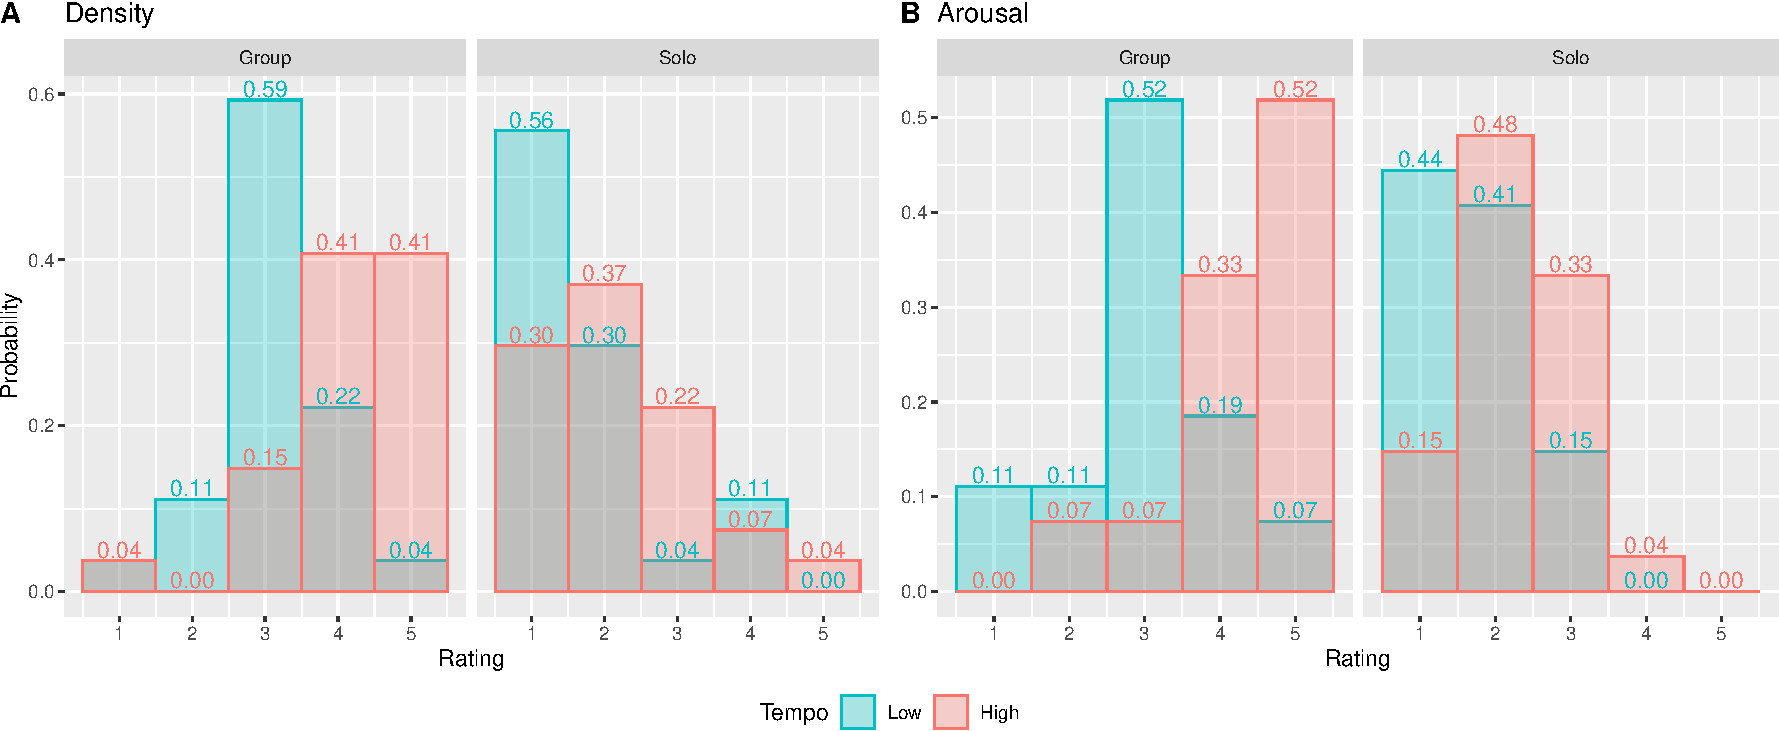
\includegraphics{Power_analysis_files/figure-latex/unnamed-chunk-7-1.pdf}
\caption{\label{fig:unnamed-chunk-7}Distribution of results from pilot data for ratings of both Density (\textbf{A}) and Arousal (\textbf{B}), by Instrumentation (Group, Solo), and Tempo (High, Low).}
\end{figure}

\hypertarget{data-simulation}{%
\subsection{Data simulation}\label{data-simulation}}

While basing a power analysis on pilot data is problematic and can bias the sample size estimation \autocite[see e.g.,][]{albersWhenPowerAnalyses2018}, we used this distribution as a starting point.

The \texttt{clmm\_generate\_data} function \autocite{bordersPowerAnalysisOrdinal2022} allows to simulate data with random and fixed effects with an ordinal outcome. In this case, we simulated data for Tempo, the within-subject variable for which there was an \emph{a-priori} prediction, replicating the distribution of the first level (Low) using a specified probability of each rating score (using the argument \texttt{control\_distribution}). The second level of that within-subject variable (Tempo = High) is generated based on a hypothesized effect (using the argument \texttt{effect}). Other important factors such as participant country and music country were randomly assigned, as there are no \emph{a-priori} predictions regarding these factors.

\hypertarget{replication-of-the-pilot-data-distribution}{%
\subsubsection{Replication of the pilot data distribution}\label{replication-of-the-pilot-data-distribution}}

To obtain distributions similar to the probabilities observed in the pilot data, we first simulated individual data for Density and Arousal ratings, separated by Instrumentation type (Group, Solo). In all cases, we simulated data from 10000 participants, and changed the value assigned to the \texttt{effect} argument until the distribution of the second level of the within-subject variable (Tempo = High) resembled the pilot data.

\begin{Shaded}
\begin{Highlighting}[]
\CommentTok{\# Density ratings for group music}
\NormalTok{dat.den.gr.PILOT }\OtherTok{\textless{}{-}} \FunctionTok{clmm\_generate\_data}\NormalTok{(}\AttributeTok{n\_participants =} \DecValTok{10000}\NormalTok{,}
                           \AttributeTok{n\_trials =} \DecValTok{3}\NormalTok{,}
                           \AttributeTok{control\_distribution =} \FunctionTok{c}\NormalTok{(.}\DecValTok{04}\NormalTok{, .}\DecValTok{11}\NormalTok{, .}\DecValTok{59}\NormalTok{, .}\DecValTok{22}\NormalTok{, .}\DecValTok{04}\NormalTok{),}
                           \AttributeTok{effect =} \FloatTok{3.2}\NormalTok{,}
                           \AttributeTok{participant\_variation =} \DecValTok{1}\NormalTok{,}
                           \AttributeTok{within\_subject =} \ConstantTok{TRUE}\NormalTok{,}
                           \AttributeTok{control\_weight =}\NormalTok{ .}\DecValTok{5}\NormalTok{) }\SpecialCharTok{|\textgreater{}}
  \FunctionTok{mutate}\NormalTok{(}\AttributeTok{group =} \FunctionTok{ifelse}\NormalTok{(group }\SpecialCharTok{==} \DecValTok{0}\NormalTok{, }\StringTok{"Low"}\NormalTok{, }\StringTok{"High"}\NormalTok{)) }\SpecialCharTok{|\textgreater{}}
\NormalTok{  dplyr}\SpecialCharTok{::}\FunctionTok{rename}\NormalTok{(}\AttributeTok{Density.tempo =}\NormalTok{ pas) }\SpecialCharTok{|\textgreater{}}
\NormalTok{  dplyr}\SpecialCharTok{::}\FunctionTok{rename}\NormalTok{(}\AttributeTok{Tempo =}\NormalTok{ group) }\SpecialCharTok{|\textgreater{}}
\NormalTok{  dplyr}\SpecialCharTok{::}\FunctionTok{rename}\NormalTok{(}\AttributeTok{Participant =}\NormalTok{ id) }\SpecialCharTok{|\textgreater{}}
  \FunctionTok{mutate}\NormalTok{(}\AttributeTok{Participant =} \FunctionTok{paste0}\NormalTok{(}\StringTok{"p"}\NormalTok{, Participant)) }\SpecialCharTok{|\textgreater{}}
  \FunctionTok{select}\NormalTok{(}\DecValTok{1}\SpecialCharTok{:}\DecValTok{3}\NormalTok{) }\SpecialCharTok{|\textgreater{}}
  \FunctionTok{mutate}\NormalTok{(}\AttributeTok{pair =} \FunctionTok{rep}\NormalTok{(}\DecValTok{1}\SpecialCharTok{:}\DecValTok{3}\NormalTok{, }\AttributeTok{times =} \DecValTok{20000}\NormalTok{)) }\SpecialCharTok{|\textgreater{}}
  \FunctionTok{mutate}\NormalTok{(}\AttributeTok{Participant.country =} \FunctionTok{rep}\NormalTok{(}\FunctionTok{rep}\NormalTok{(}\FunctionTok{c}\NormalTok{(}\StringTok{"Iran"}\NormalTok{, }\StringTok{"Canada"}\NormalTok{, }\StringTok{"Japan"}\NormalTok{), }\AttributeTok{each =} \DecValTok{10000}\NormalTok{), }\DecValTok{2}\NormalTok{)) }\SpecialCharTok{|\textgreater{}}
  \FunctionTok{mutate}\NormalTok{(}\AttributeTok{Music.country =} \FunctionTok{rep}\NormalTok{(}\FunctionTok{c}\NormalTok{(}\StringTok{"Iran"}\NormalTok{, }\StringTok{"Canada"}\NormalTok{, }\StringTok{"Japan"}\NormalTok{), }\AttributeTok{times =} \DecValTok{20000}\NormalTok{)) }\SpecialCharTok{|\textgreater{}}
  \FunctionTok{mutate}\NormalTok{(}\AttributeTok{Solo.group =} \FunctionTok{rep}\NormalTok{(}\StringTok{"Group"}\NormalTok{, }\AttributeTok{TIMES =} \DecValTok{60000}\NormalTok{)) }\SpecialCharTok{|\textgreater{}}
  \FunctionTok{select}\NormalTok{(}\FunctionTok{c}\NormalTok{(}\DecValTok{1}\NormalTok{,}\DecValTok{6}\NormalTok{,}\DecValTok{5}\NormalTok{,}\DecValTok{2}\NormalTok{,}\DecValTok{7}\NormalTok{,}\DecValTok{3}\NormalTok{))}

\CommentTok{\# Density ratings for solo music}
\NormalTok{dat.den.so.PILOT }\OtherTok{\textless{}{-}} \FunctionTok{clmm\_generate\_data}\NormalTok{(}\AttributeTok{n\_participants =} \DecValTok{10000}\NormalTok{,}
                                 \AttributeTok{n\_trials =} \DecValTok{3}\NormalTok{,}
                                 \AttributeTok{control\_distribution =} \FunctionTok{c}\NormalTok{(.}\DecValTok{55}\NormalTok{, .}\DecValTok{30}\NormalTok{, .}\DecValTok{04}\NormalTok{, .}\DecValTok{10}\NormalTok{, .}\DecValTok{01}\NormalTok{),}
                                 \AttributeTok{effect =} \FloatTok{1.2}\NormalTok{,}
                                 \AttributeTok{participant\_variation =} \DecValTok{1}\NormalTok{,}
                                 \AttributeTok{within\_subject =} \ConstantTok{TRUE}\NormalTok{,}
                                 \AttributeTok{control\_weight =}\NormalTok{ .}\DecValTok{5}\NormalTok{) }\SpecialCharTok{|\textgreater{}}
  \FunctionTok{mutate}\NormalTok{(}\AttributeTok{group =} \FunctionTok{ifelse}\NormalTok{(group }\SpecialCharTok{==} \DecValTok{0}\NormalTok{, }\StringTok{"Low"}\NormalTok{, }\StringTok{"High"}\NormalTok{)) }\SpecialCharTok{|\textgreater{}}
\NormalTok{  dplyr}\SpecialCharTok{::}\FunctionTok{rename}\NormalTok{(}\AttributeTok{Density.tempo =}\NormalTok{ pas) }\SpecialCharTok{|\textgreater{}}
\NormalTok{  dplyr}\SpecialCharTok{::}\FunctionTok{rename}\NormalTok{(}\AttributeTok{Tempo =}\NormalTok{ group) }\SpecialCharTok{|\textgreater{}}
\NormalTok{  dplyr}\SpecialCharTok{::}\FunctionTok{rename}\NormalTok{(}\AttributeTok{Participant =}\NormalTok{ id) }\SpecialCharTok{|\textgreater{}}
  \FunctionTok{mutate}\NormalTok{(}\AttributeTok{Participant =} \FunctionTok{paste0}\NormalTok{(}\StringTok{"p"}\NormalTok{, Participant)) }\SpecialCharTok{|\textgreater{}}
  \FunctionTok{select}\NormalTok{(}\DecValTok{1}\SpecialCharTok{:}\DecValTok{3}\NormalTok{) }\SpecialCharTok{|\textgreater{}}
  \FunctionTok{mutate}\NormalTok{(}\AttributeTok{pair =} \FunctionTok{rep}\NormalTok{(}\DecValTok{1}\SpecialCharTok{:}\DecValTok{3}\NormalTok{, }\AttributeTok{times =} \DecValTok{20000}\NormalTok{)) }\SpecialCharTok{|\textgreater{}}
  \FunctionTok{mutate}\NormalTok{(}\AttributeTok{Participant.country =} \FunctionTok{rep}\NormalTok{(}\FunctionTok{rep}\NormalTok{(}\FunctionTok{c}\NormalTok{(}\StringTok{"Iran"}\NormalTok{, }\StringTok{"Canada"}\NormalTok{, }\StringTok{"Japan"}\NormalTok{), }\AttributeTok{each =} \DecValTok{10000}\NormalTok{), }\DecValTok{2}\NormalTok{)) }\SpecialCharTok{|\textgreater{}}
  \FunctionTok{mutate}\NormalTok{(}\AttributeTok{Music.country =} \FunctionTok{rep}\NormalTok{(}\FunctionTok{c}\NormalTok{(}\StringTok{"Iran"}\NormalTok{, }\StringTok{"Canada"}\NormalTok{, }\StringTok{"Japan"}\NormalTok{), }\AttributeTok{times =} \DecValTok{20000}\NormalTok{)) }\SpecialCharTok{|\textgreater{}}
  \FunctionTok{mutate}\NormalTok{(}\AttributeTok{Solo.group =} \FunctionTok{rep}\NormalTok{(}\StringTok{"Solo"}\NormalTok{, }\AttributeTok{TIMES =} \DecValTok{60000}\NormalTok{)) }\SpecialCharTok{|\textgreater{}}
  \FunctionTok{select}\NormalTok{(}\FunctionTok{c}\NormalTok{(}\DecValTok{1}\NormalTok{,}\DecValTok{6}\NormalTok{,}\DecValTok{5}\NormalTok{,}\DecValTok{2}\NormalTok{,}\DecValTok{7}\NormalTok{,}\DecValTok{3}\NormalTok{))}

\CommentTok{\# Arousal ratings for group music}
\NormalTok{dat.aro.gr.PILOT }\OtherTok{\textless{}{-}} \FunctionTok{clmm\_generate\_data}\NormalTok{(}\AttributeTok{n\_participants =} \DecValTok{10000}\NormalTok{,}
                                 \AttributeTok{n\_trials =} \DecValTok{3}\NormalTok{,}
                                 \AttributeTok{control\_distribution =} \FunctionTok{c}\NormalTok{(.}\DecValTok{11}\NormalTok{, .}\DecValTok{11}\NormalTok{, .}\DecValTok{52}\NormalTok{, .}\DecValTok{19}\NormalTok{, .}\DecValTok{07}\NormalTok{),}
                                 \AttributeTok{effect =} \FloatTok{3.1}\NormalTok{,}
                                 \AttributeTok{participant\_variation =} \DecValTok{1}\NormalTok{,}
                                 \AttributeTok{within\_subject =} \ConstantTok{TRUE}\NormalTok{,}
                                 \AttributeTok{control\_weight =}\NormalTok{ .}\DecValTok{5}\NormalTok{) }\SpecialCharTok{|\textgreater{}}
  \FunctionTok{mutate}\NormalTok{(}\AttributeTok{group =} \FunctionTok{ifelse}\NormalTok{(group }\SpecialCharTok{==} \DecValTok{0}\NormalTok{, }\StringTok{"Low"}\NormalTok{, }\StringTok{"High"}\NormalTok{)) }\SpecialCharTok{|\textgreater{}}
\NormalTok{  dplyr}\SpecialCharTok{::}\FunctionTok{rename}\NormalTok{(}\AttributeTok{Arousal.tempo =}\NormalTok{ pas) }\SpecialCharTok{|\textgreater{}}
\NormalTok{  dplyr}\SpecialCharTok{::}\FunctionTok{rename}\NormalTok{(}\AttributeTok{Tempo =}\NormalTok{ group) }\SpecialCharTok{|\textgreater{}}
\NormalTok{  dplyr}\SpecialCharTok{::}\FunctionTok{rename}\NormalTok{(}\AttributeTok{Participant =}\NormalTok{ id) }\SpecialCharTok{|\textgreater{}}
  \FunctionTok{mutate}\NormalTok{(}\AttributeTok{Participant =} \FunctionTok{paste0}\NormalTok{(}\StringTok{"p"}\NormalTok{, Participant)) }\SpecialCharTok{|\textgreater{}}
  \FunctionTok{select}\NormalTok{(}\DecValTok{1}\SpecialCharTok{:}\DecValTok{3}\NormalTok{) }\SpecialCharTok{|\textgreater{}}
  \FunctionTok{mutate}\NormalTok{(}\AttributeTok{pair =} \FunctionTok{rep}\NormalTok{(}\DecValTok{1}\SpecialCharTok{:}\DecValTok{3}\NormalTok{, }\AttributeTok{times =} \DecValTok{20000}\NormalTok{)) }\SpecialCharTok{|\textgreater{}}
  \FunctionTok{mutate}\NormalTok{(}\AttributeTok{Participant.country =} \FunctionTok{rep}\NormalTok{(}\FunctionTok{rep}\NormalTok{(}\FunctionTok{c}\NormalTok{(}\StringTok{"Iran"}\NormalTok{, }\StringTok{"Canada"}\NormalTok{, }\StringTok{"Japan"}\NormalTok{), }\AttributeTok{each =} \DecValTok{10000}\NormalTok{), }\DecValTok{2}\NormalTok{)) }\SpecialCharTok{|\textgreater{}}
  \FunctionTok{mutate}\NormalTok{(}\AttributeTok{Music.country =} \FunctionTok{rep}\NormalTok{(}\FunctionTok{c}\NormalTok{(}\StringTok{"Iran"}\NormalTok{, }\StringTok{"Canada"}\NormalTok{, }\StringTok{"Japan"}\NormalTok{), }\AttributeTok{times =} \DecValTok{20000}\NormalTok{)) }\SpecialCharTok{|\textgreater{}}
  \FunctionTok{mutate}\NormalTok{(}\AttributeTok{Solo.group =} \FunctionTok{rep}\NormalTok{(}\StringTok{"Group"}\NormalTok{, }\AttributeTok{TIMES =} \DecValTok{60000}\NormalTok{)) }\SpecialCharTok{|\textgreater{}}
  \FunctionTok{select}\NormalTok{(}\FunctionTok{c}\NormalTok{(}\DecValTok{1}\NormalTok{,}\DecValTok{6}\NormalTok{,}\DecValTok{5}\NormalTok{,}\DecValTok{2}\NormalTok{,}\DecValTok{7}\NormalTok{,}\DecValTok{3}\NormalTok{))}

\CommentTok{\# Arousal ratings for solo music}
\NormalTok{dat.aro.so.PILOT }\OtherTok{\textless{}{-}} \FunctionTok{clmm\_generate\_data}\NormalTok{(}\AttributeTok{n\_participants =} \DecValTok{10000}\NormalTok{,}
                                 \AttributeTok{n\_trials =} \DecValTok{3}\NormalTok{,}
                                 \AttributeTok{control\_distribution =} \FunctionTok{c}\NormalTok{(.}\DecValTok{43}\NormalTok{, .}\DecValTok{41}\NormalTok{, .}\DecValTok{14}\NormalTok{, .}\DecValTok{01}\NormalTok{, .}\DecValTok{01}\NormalTok{),}
                                 \AttributeTok{effect =} \FloatTok{1.6}\NormalTok{,}
                                 \AttributeTok{participant\_variation =} \DecValTok{1}\NormalTok{,}
                                 \AttributeTok{within\_subject =} \ConstantTok{TRUE}\NormalTok{,}
                                 \AttributeTok{control\_weight =}\NormalTok{ .}\DecValTok{5}\NormalTok{) }\SpecialCharTok{|\textgreater{}}
  \FunctionTok{mutate}\NormalTok{(}\AttributeTok{group =} \FunctionTok{ifelse}\NormalTok{(group }\SpecialCharTok{==} \DecValTok{0}\NormalTok{, }\StringTok{"Low"}\NormalTok{, }\StringTok{"High"}\NormalTok{)) }\SpecialCharTok{|\textgreater{}}
\NormalTok{  dplyr}\SpecialCharTok{::}\FunctionTok{rename}\NormalTok{(}\AttributeTok{Arousal.tempo =}\NormalTok{ pas) }\SpecialCharTok{|\textgreater{}}
\NormalTok{  dplyr}\SpecialCharTok{::}\FunctionTok{rename}\NormalTok{(}\AttributeTok{Tempo =}\NormalTok{ group) }\SpecialCharTok{|\textgreater{}}
\NormalTok{  dplyr}\SpecialCharTok{::}\FunctionTok{rename}\NormalTok{(}\AttributeTok{Participant =}\NormalTok{ id) }\SpecialCharTok{|\textgreater{}}
  \FunctionTok{mutate}\NormalTok{(}\AttributeTok{Participant =} \FunctionTok{paste0}\NormalTok{(}\StringTok{"p"}\NormalTok{, Participant)) }\SpecialCharTok{|\textgreater{}}
  \FunctionTok{select}\NormalTok{(}\DecValTok{1}\SpecialCharTok{:}\DecValTok{3}\NormalTok{) }\SpecialCharTok{|\textgreater{}}
  \FunctionTok{mutate}\NormalTok{(}\AttributeTok{pair =} \FunctionTok{rep}\NormalTok{(}\DecValTok{1}\SpecialCharTok{:}\DecValTok{3}\NormalTok{, }\AttributeTok{times =} \DecValTok{20000}\NormalTok{)) }\SpecialCharTok{|\textgreater{}}
  \FunctionTok{mutate}\NormalTok{(}\AttributeTok{Participant.country =} \FunctionTok{rep}\NormalTok{(}\FunctionTok{rep}\NormalTok{(}\FunctionTok{c}\NormalTok{(}\StringTok{"Iran"}\NormalTok{, }\StringTok{"Canada"}\NormalTok{, }\StringTok{"Japan"}\NormalTok{), }\AttributeTok{each =} \DecValTok{10000}\NormalTok{), }\DecValTok{2}\NormalTok{)) }\SpecialCharTok{|\textgreater{}}
  \FunctionTok{mutate}\NormalTok{(}\AttributeTok{Music.country =} \FunctionTok{rep}\NormalTok{(}\FunctionTok{c}\NormalTok{(}\StringTok{"Iran"}\NormalTok{, }\StringTok{"Canada"}\NormalTok{, }\StringTok{"Japan"}\NormalTok{), }\AttributeTok{times =} \DecValTok{20000}\NormalTok{)) }\SpecialCharTok{|\textgreater{}}
  \FunctionTok{mutate}\NormalTok{(}\AttributeTok{Solo.group =} \FunctionTok{rep}\NormalTok{(}\StringTok{"Solo"}\NormalTok{, }\AttributeTok{TIMES =} \DecValTok{60000}\NormalTok{)) }\SpecialCharTok{|\textgreater{}}
  \FunctionTok{select}\NormalTok{(}\FunctionTok{c}\NormalTok{(}\DecValTok{1}\NormalTok{,}\DecValTok{6}\NormalTok{,}\DecValTok{5}\NormalTok{,}\DecValTok{2}\NormalTok{,}\DecValTok{7}\NormalTok{,}\DecValTok{3}\NormalTok{))}
\end{Highlighting}
\end{Shaded}

We then merged these four data frames to obtain a simulated data frame.

\begin{Shaded}
\begin{Highlighting}[]
\NormalTok{dat.sim.PILOT }\OtherTok{\textless{}{-}} \FunctionTok{left\_join}\NormalTok{(}\FunctionTok{bind\_rows}\NormalTok{(dat.den.gr.PILOT, dat.den.so.PILOT),}
                           \FunctionTok{bind\_rows}\NormalTok{(dat.aro.gr.PILOT, dat.aro.so.PILOT),}
                           \AttributeTok{relationship =} \StringTok{"many{-}to{-}many"}\NormalTok{) }\SpecialCharTok{|\textgreater{}} 
  \FunctionTok{mutate}\NormalTok{(}\AttributeTok{Tempo =} \FunctionTok{fct\_relevel}\NormalTok{(Tempo, }\FunctionTok{c}\NormalTok{(}\StringTok{"Low"}\NormalTok{, }\StringTok{"High"}\NormalTok{)))}
\end{Highlighting}
\end{Shaded}

The distribution of this replication of the pilot data distribution is represented in \ref{fig:pilot-rep}

\begin{Shaded}
\begin{Highlighting}[]
\CommentTok{\# Plot distribution of results for density ratings}
\NormalTok{p2a }\OtherTok{\textless{}{-}} \FunctionTok{ggplot}\NormalTok{(dat.sim.PILOT, }\FunctionTok{aes}\NormalTok{(}\AttributeTok{x =}\NormalTok{ Density.tempo, }\AttributeTok{y =} \FunctionTok{after\_stat}\NormalTok{(density),}
                                 \AttributeTok{fill =}\NormalTok{ Tempo, }\AttributeTok{color =}\NormalTok{ Tempo)) }\SpecialCharTok{+}
  \FunctionTok{scale\_fill\_hue}\NormalTok{(}\AttributeTok{direction =} \SpecialCharTok{{-}}\DecValTok{1}\NormalTok{) }\SpecialCharTok{+} \FunctionTok{scale\_colour\_hue}\NormalTok{(}\AttributeTok{direction =} \SpecialCharTok{{-}}\DecValTok{1}\NormalTok{) }\SpecialCharTok{+}
  \FunctionTok{geom\_histogram}\NormalTok{(}\AttributeTok{alpha =} \FloatTok{0.3}\NormalTok{, }\AttributeTok{position =} \StringTok{"identity"}\NormalTok{, }\AttributeTok{binwidth =} \DecValTok{1}\NormalTok{) }\SpecialCharTok{+}
  \FunctionTok{labs}\NormalTok{(}\AttributeTok{y=} \StringTok{"Probability"}\NormalTok{, }\AttributeTok{x =} \StringTok{"Rating"}\NormalTok{) }\SpecialCharTok{+}
  \FunctionTok{geom\_text}\NormalTok{(}\FunctionTok{aes}\NormalTok{(}\AttributeTok{label =} \FunctionTok{format}\NormalTok{(}\FunctionTok{after\_stat}\NormalTok{(density), }\AttributeTok{digits =} \DecValTok{1}\NormalTok{), }\AttributeTok{y=} \FunctionTok{after\_stat}\NormalTok{(density)), }
            \AttributeTok{stat=} \StringTok{"bin"}\NormalTok{, }\AttributeTok{binwidth =} \DecValTok{1}\NormalTok{, }
            \AttributeTok{vjust =} \SpecialCharTok{{-}}\FloatTok{0.2}\NormalTok{,}
            \AttributeTok{show.legend =} \ConstantTok{FALSE}\NormalTok{) }\SpecialCharTok{+}
  \FunctionTok{facet\_wrap}\NormalTok{(}\SpecialCharTok{\textasciitilde{}}\NormalTok{Solo.group)}

\CommentTok{\# Plot distribution of results for arousal ratings}
\NormalTok{p2b }\OtherTok{\textless{}{-}} \FunctionTok{ggplot}\NormalTok{(dat.sim.PILOT, }\FunctionTok{aes}\NormalTok{(}\AttributeTok{x =}\NormalTok{ Arousal.tempo, }\AttributeTok{y =} \FunctionTok{after\_stat}\NormalTok{(density),}
                                 \AttributeTok{fill =}\NormalTok{ Tempo, }\AttributeTok{color =}\NormalTok{ Tempo)) }\SpecialCharTok{+}
  \FunctionTok{scale\_fill\_hue}\NormalTok{(}\AttributeTok{direction =} \SpecialCharTok{{-}}\DecValTok{1}\NormalTok{) }\SpecialCharTok{+} \FunctionTok{scale\_colour\_hue}\NormalTok{(}\AttributeTok{direction =} \SpecialCharTok{{-}}\DecValTok{1}\NormalTok{) }\SpecialCharTok{+}
  \FunctionTok{geom\_histogram}\NormalTok{(}\AttributeTok{alpha =} \FloatTok{0.3}\NormalTok{, }\AttributeTok{position =} \StringTok{"identity"}\NormalTok{, }\AttributeTok{binwidth =} \DecValTok{1}\NormalTok{) }\SpecialCharTok{+}
  \FunctionTok{labs}\NormalTok{(}\AttributeTok{y=} \ConstantTok{NULL}\NormalTok{, }\AttributeTok{x =} \StringTok{"Rating"}\NormalTok{) }\SpecialCharTok{+}
  \FunctionTok{geom\_text}\NormalTok{(}\FunctionTok{aes}\NormalTok{(}\AttributeTok{label =} \FunctionTok{format}\NormalTok{(}\FunctionTok{after\_stat}\NormalTok{(density), }\AttributeTok{digits =} \DecValTok{1}\NormalTok{), }\AttributeTok{y=} \FunctionTok{after\_stat}\NormalTok{(density)), }
            \AttributeTok{stat=} \StringTok{"bin"}\NormalTok{, }\AttributeTok{binwidth =} \DecValTok{1}\NormalTok{, }
            \AttributeTok{vjust =} \SpecialCharTok{{-}}\FloatTok{0.2}\NormalTok{,}
            \AttributeTok{show.legend =} \ConstantTok{FALSE}\NormalTok{) }\SpecialCharTok{+}
  \FunctionTok{facet\_wrap}\NormalTok{(}\SpecialCharTok{\textasciitilde{}}\NormalTok{Solo.group)}

\CommentTok{\# Arrange plots}
\NormalTok{p2 }\OtherTok{\textless{}{-}} \FunctionTok{ggarrange}\NormalTok{(p2a }\SpecialCharTok{+}
                  \FunctionTok{labs}\NormalTok{(}\AttributeTok{subtitle =} \StringTok{"Density"}\NormalTok{), }
\NormalTok{                p2b  }\SpecialCharTok{+}
                  \FunctionTok{labs}\NormalTok{(}\AttributeTok{subtitle =} \StringTok{"Arousal"}\NormalTok{),}
                \AttributeTok{common.legend =} \ConstantTok{TRUE}\NormalTok{,}
                \AttributeTok{legend =} \StringTok{"bottom"}\NormalTok{,}
                \AttributeTok{labels =} \StringTok{"AUTO"}\NormalTok{)}
\NormalTok{p2}
\end{Highlighting}
\end{Shaded}

\begin{figure}
\centering
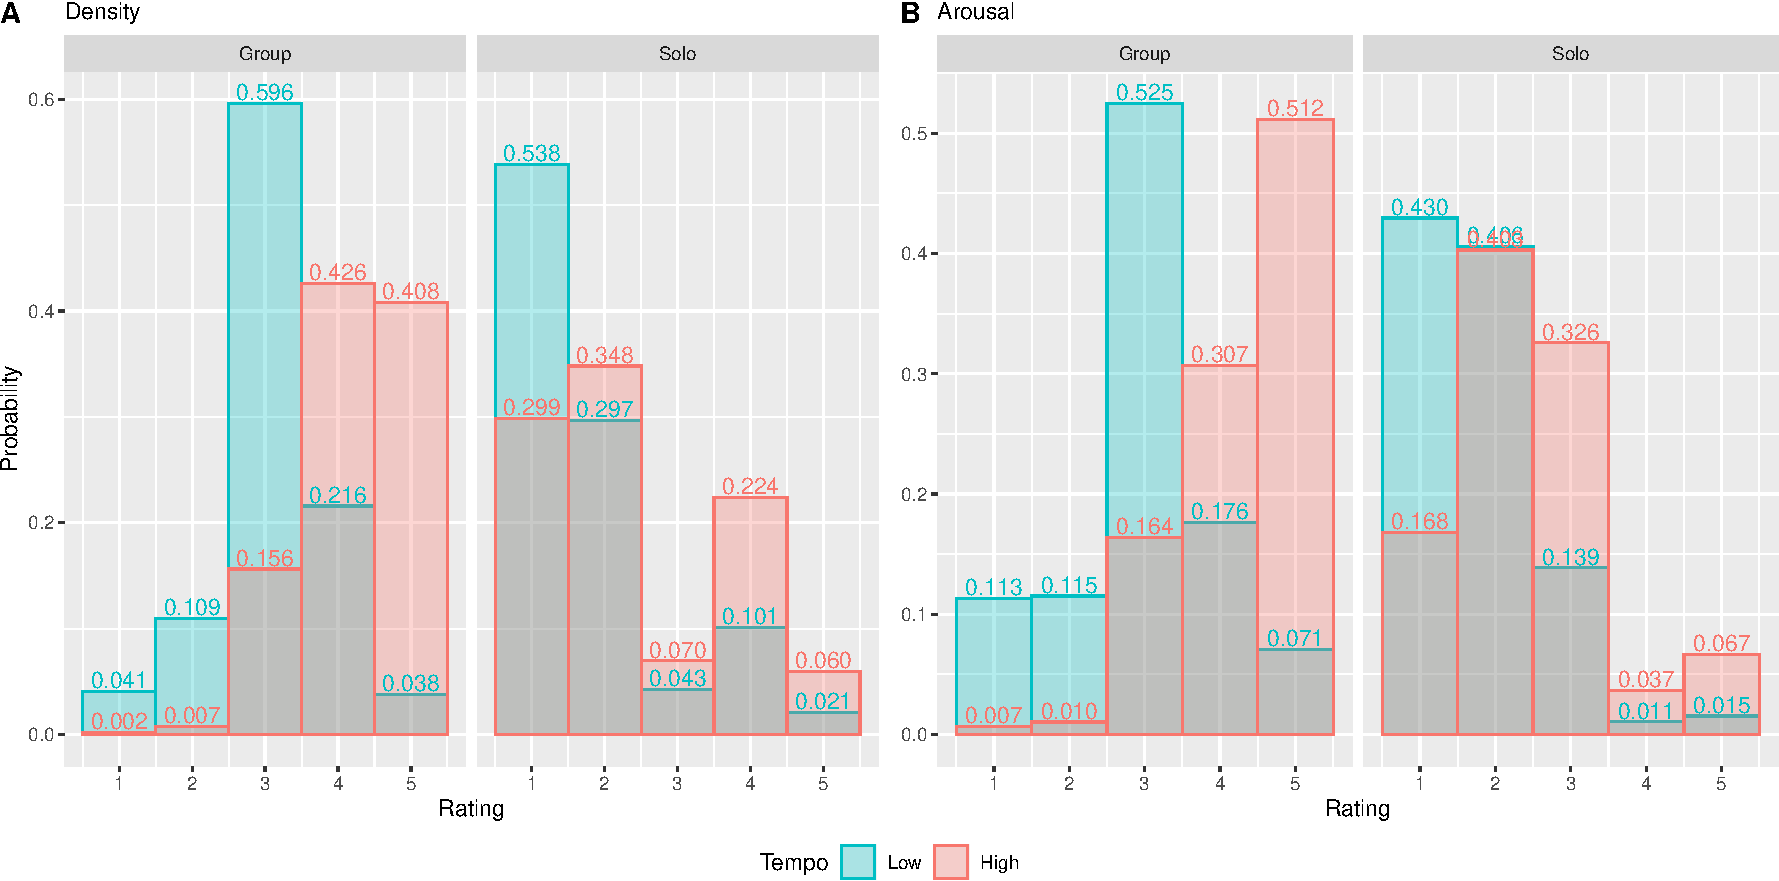
\includegraphics{Power_analysis_files/figure-latex/pilot-rep-1.pdf}
\caption{\label{fig:pilot-rep}Distribution of results from a simulated replication of the pilot data distribution for ratings of both Density (\textbf{A}) and Arousal (\textbf{B}), by Instrumentation (Group, Solo), and Tempo (High, Low).}
\end{figure}

\hypertarget{simulation-of-data-with-a-more-conservative-effect}{%
\subsubsection{Simulation of data with a more conservative effect}\label{simulation-of-data-with-a-more-conservative-effect}}

While the data simulated in the previous section resembled the distribution of the pilot data, using these data would be problematic for at least two reasons:

First, the effects of Tempo were extremely large (3.2, 1.2, 3.1, 1.6), particularly for ratings of Group instrumentation (3.2, and 3.1). With such differences, a very high statistical power of about \(1 - \beta = 0.95\) can be achieved with 2 or 3 participants. And second, as mentioned before, estimating effects from pilot data is problematic, as it biases the results \autocite{albersWhenPowerAnalyses2018}.

For this reason, we decided to maintain the distributions of probabilities for the first Tempo level (Low), as it is a good starting point to estimate the distribution of ratings that participants would assign, but simulated the second level (Tempo = High) with a much more conservative effect of 1 in all cases.

\begin{Shaded}
\begin{Highlighting}[]
\CommentTok{\# Density ratings for group music}
\NormalTok{dat.den.gr }\OtherTok{\textless{}{-}} \FunctionTok{clmm\_generate\_data}\NormalTok{(}\AttributeTok{n\_participants =} \DecValTok{10000}\NormalTok{,}
                                 \AttributeTok{n\_trials =} \DecValTok{3}\NormalTok{,}
                                 \AttributeTok{control\_distribution =} \FunctionTok{c}\NormalTok{(.}\DecValTok{04}\NormalTok{, .}\DecValTok{11}\NormalTok{, .}\DecValTok{59}\NormalTok{, .}\DecValTok{22}\NormalTok{, .}\DecValTok{04}\NormalTok{),}
                                 \AttributeTok{effect =} \DecValTok{1}\NormalTok{,}
                                 \AttributeTok{participant\_variation =} \DecValTok{1}\NormalTok{,}
                                 \AttributeTok{within\_subject =} \ConstantTok{TRUE}\NormalTok{,}
                                 \AttributeTok{control\_weight =}\NormalTok{ .}\DecValTok{5}\NormalTok{) }\SpecialCharTok{|\textgreater{}}
  \FunctionTok{mutate}\NormalTok{(}\AttributeTok{group =} \FunctionTok{ifelse}\NormalTok{(group }\SpecialCharTok{==} \DecValTok{0}\NormalTok{, }\StringTok{"Low"}\NormalTok{, }\StringTok{"High"}\NormalTok{)) }\SpecialCharTok{|\textgreater{}}
\NormalTok{  dplyr}\SpecialCharTok{::}\FunctionTok{rename}\NormalTok{(}\AttributeTok{Density.tempo =}\NormalTok{ pas) }\SpecialCharTok{|\textgreater{}}
\NormalTok{  dplyr}\SpecialCharTok{::}\FunctionTok{rename}\NormalTok{(}\AttributeTok{Tempo =}\NormalTok{ group) }\SpecialCharTok{|\textgreater{}}
\NormalTok{  dplyr}\SpecialCharTok{::}\FunctionTok{rename}\NormalTok{(}\AttributeTok{Participant =}\NormalTok{ id) }\SpecialCharTok{|\textgreater{}}
  \FunctionTok{mutate}\NormalTok{(}\AttributeTok{Participant =} \FunctionTok{paste0}\NormalTok{(}\StringTok{"p"}\NormalTok{, Participant)) }\SpecialCharTok{|\textgreater{}}
  \FunctionTok{select}\NormalTok{(}\DecValTok{1}\SpecialCharTok{:}\DecValTok{3}\NormalTok{) }\SpecialCharTok{|\textgreater{}}
  \FunctionTok{mutate}\NormalTok{(}\AttributeTok{pair =} \FunctionTok{rep}\NormalTok{(}\DecValTok{1}\SpecialCharTok{:}\DecValTok{3}\NormalTok{, }\AttributeTok{times =} \DecValTok{20000}\NormalTok{)) }\SpecialCharTok{|\textgreater{}}
  \FunctionTok{mutate}\NormalTok{(}\AttributeTok{Participant.country =} \FunctionTok{rep}\NormalTok{(}\FunctionTok{rep}\NormalTok{(}\FunctionTok{c}\NormalTok{(}\StringTok{"Iran"}\NormalTok{, }\StringTok{"Canada"}\NormalTok{, }\StringTok{"Japan"}\NormalTok{), }\AttributeTok{each =} \DecValTok{10000}\NormalTok{), }\DecValTok{2}\NormalTok{)) }\SpecialCharTok{|\textgreater{}}
  \FunctionTok{mutate}\NormalTok{(}\AttributeTok{Music.country =} \FunctionTok{rep}\NormalTok{(}\FunctionTok{c}\NormalTok{(}\StringTok{"Iran"}\NormalTok{, }\StringTok{"Canada"}\NormalTok{, }\StringTok{"Japan"}\NormalTok{), }\AttributeTok{times =} \DecValTok{20000}\NormalTok{)) }\SpecialCharTok{|\textgreater{}}
  \FunctionTok{mutate}\NormalTok{(}\AttributeTok{Solo.group =} \FunctionTok{rep}\NormalTok{(}\StringTok{"Group"}\NormalTok{, }\AttributeTok{TIMES =} \DecValTok{60000}\NormalTok{)) }\SpecialCharTok{|\textgreater{}}
  \FunctionTok{select}\NormalTok{(}\FunctionTok{c}\NormalTok{(}\DecValTok{1}\NormalTok{,}\DecValTok{6}\NormalTok{,}\DecValTok{5}\NormalTok{,}\DecValTok{2}\NormalTok{,}\DecValTok{7}\NormalTok{,}\DecValTok{3}\NormalTok{))}

\CommentTok{\# Density ratings for solo music}
\NormalTok{dat.den.so }\OtherTok{\textless{}{-}} \FunctionTok{clmm\_generate\_data}\NormalTok{(}\AttributeTok{n\_participants =} \DecValTok{10000}\NormalTok{,}
                                 \AttributeTok{n\_trials =} \DecValTok{3}\NormalTok{,}
                                 \AttributeTok{control\_distribution =} \FunctionTok{c}\NormalTok{(.}\DecValTok{55}\NormalTok{, .}\DecValTok{30}\NormalTok{, .}\DecValTok{04}\NormalTok{, .}\DecValTok{10}\NormalTok{, .}\DecValTok{01}\NormalTok{),}
                                 \AttributeTok{effect =} \DecValTok{1}\NormalTok{,}
                                 \AttributeTok{participant\_variation =} \DecValTok{1}\NormalTok{,}
                                 \AttributeTok{within\_subject =} \ConstantTok{TRUE}\NormalTok{,}
                                 \AttributeTok{control\_weight =}\NormalTok{ .}\DecValTok{5}\NormalTok{) }\SpecialCharTok{|\textgreater{}}
  \FunctionTok{mutate}\NormalTok{(}\AttributeTok{group =} \FunctionTok{ifelse}\NormalTok{(group }\SpecialCharTok{==} \DecValTok{0}\NormalTok{, }\StringTok{"Low"}\NormalTok{, }\StringTok{"High"}\NormalTok{)) }\SpecialCharTok{|\textgreater{}}
\NormalTok{  dplyr}\SpecialCharTok{::}\FunctionTok{rename}\NormalTok{(}\AttributeTok{Density.tempo =}\NormalTok{ pas) }\SpecialCharTok{|\textgreater{}}
\NormalTok{  dplyr}\SpecialCharTok{::}\FunctionTok{rename}\NormalTok{(}\AttributeTok{Tempo =}\NormalTok{ group) }\SpecialCharTok{|\textgreater{}}
\NormalTok{  dplyr}\SpecialCharTok{::}\FunctionTok{rename}\NormalTok{(}\AttributeTok{Participant =}\NormalTok{ id) }\SpecialCharTok{|\textgreater{}}
  \FunctionTok{mutate}\NormalTok{(}\AttributeTok{Participant =} \FunctionTok{paste0}\NormalTok{(}\StringTok{"p"}\NormalTok{, Participant)) }\SpecialCharTok{|\textgreater{}}
  \FunctionTok{select}\NormalTok{(}\DecValTok{1}\SpecialCharTok{:}\DecValTok{3}\NormalTok{) }\SpecialCharTok{|\textgreater{}}
  \FunctionTok{mutate}\NormalTok{(}\AttributeTok{pair =} \FunctionTok{rep}\NormalTok{(}\DecValTok{1}\SpecialCharTok{:}\DecValTok{3}\NormalTok{, }\AttributeTok{times =} \DecValTok{20000}\NormalTok{)) }\SpecialCharTok{|\textgreater{}}
  \FunctionTok{mutate}\NormalTok{(}\AttributeTok{Participant.country =} \FunctionTok{rep}\NormalTok{(}\FunctionTok{rep}\NormalTok{(}\FunctionTok{c}\NormalTok{(}\StringTok{"Iran"}\NormalTok{, }\StringTok{"Canada"}\NormalTok{, }\StringTok{"Japan"}\NormalTok{), }\AttributeTok{each =} \DecValTok{10000}\NormalTok{), }\DecValTok{2}\NormalTok{)) }\SpecialCharTok{|\textgreater{}}
  \FunctionTok{mutate}\NormalTok{(}\AttributeTok{Music.country =} \FunctionTok{rep}\NormalTok{(}\FunctionTok{c}\NormalTok{(}\StringTok{"Iran"}\NormalTok{, }\StringTok{"Canada"}\NormalTok{, }\StringTok{"Japan"}\NormalTok{), }\AttributeTok{times =} \DecValTok{20000}\NormalTok{)) }\SpecialCharTok{|\textgreater{}}
  \FunctionTok{mutate}\NormalTok{(}\AttributeTok{Solo.group =} \FunctionTok{rep}\NormalTok{(}\StringTok{"Solo"}\NormalTok{, }\AttributeTok{TIMES =} \DecValTok{60000}\NormalTok{)) }\SpecialCharTok{|\textgreater{}}
  \FunctionTok{select}\NormalTok{(}\FunctionTok{c}\NormalTok{(}\DecValTok{1}\NormalTok{,}\DecValTok{6}\NormalTok{,}\DecValTok{5}\NormalTok{,}\DecValTok{2}\NormalTok{,}\DecValTok{7}\NormalTok{,}\DecValTok{3}\NormalTok{))}

\CommentTok{\# Arousal ratings for group music}
\NormalTok{dat.aro.gr }\OtherTok{\textless{}{-}} \FunctionTok{clmm\_generate\_data}\NormalTok{(}\AttributeTok{n\_participants =} \DecValTok{10000}\NormalTok{,}
                                 \AttributeTok{n\_trials =} \DecValTok{3}\NormalTok{,}
                                 \AttributeTok{control\_distribution =} \FunctionTok{c}\NormalTok{(.}\DecValTok{11}\NormalTok{, .}\DecValTok{11}\NormalTok{, .}\DecValTok{52}\NormalTok{, .}\DecValTok{19}\NormalTok{, .}\DecValTok{07}\NormalTok{),}
                                 \AttributeTok{effect =} \DecValTok{1}\NormalTok{,}
                                 \AttributeTok{participant\_variation =} \DecValTok{1}\NormalTok{,}
                                 \AttributeTok{within\_subject =} \ConstantTok{TRUE}\NormalTok{,}
                                 \AttributeTok{control\_weight =}\NormalTok{ .}\DecValTok{5}\NormalTok{) }\SpecialCharTok{|\textgreater{}}
  \FunctionTok{mutate}\NormalTok{(}\AttributeTok{group =} \FunctionTok{ifelse}\NormalTok{(group }\SpecialCharTok{==} \DecValTok{0}\NormalTok{, }\StringTok{"Low"}\NormalTok{, }\StringTok{"High"}\NormalTok{)) }\SpecialCharTok{|\textgreater{}}
\NormalTok{  dplyr}\SpecialCharTok{::}\FunctionTok{rename}\NormalTok{(}\AttributeTok{Arousal.tempo =}\NormalTok{ pas) }\SpecialCharTok{|\textgreater{}}
\NormalTok{  dplyr}\SpecialCharTok{::}\FunctionTok{rename}\NormalTok{(}\AttributeTok{Tempo =}\NormalTok{ group) }\SpecialCharTok{|\textgreater{}}
\NormalTok{  dplyr}\SpecialCharTok{::}\FunctionTok{rename}\NormalTok{(}\AttributeTok{Participant =}\NormalTok{ id) }\SpecialCharTok{|\textgreater{}}
  \FunctionTok{mutate}\NormalTok{(}\AttributeTok{Participant =} \FunctionTok{paste0}\NormalTok{(}\StringTok{"p"}\NormalTok{, Participant)) }\SpecialCharTok{|\textgreater{}}
  \FunctionTok{select}\NormalTok{(}\DecValTok{1}\SpecialCharTok{:}\DecValTok{3}\NormalTok{) }\SpecialCharTok{|\textgreater{}}
  \FunctionTok{mutate}\NormalTok{(}\AttributeTok{pair =} \FunctionTok{rep}\NormalTok{(}\DecValTok{1}\SpecialCharTok{:}\DecValTok{3}\NormalTok{, }\AttributeTok{times =} \DecValTok{20000}\NormalTok{)) }\SpecialCharTok{|\textgreater{}}
  \FunctionTok{mutate}\NormalTok{(}\AttributeTok{Participant.country =} \FunctionTok{rep}\NormalTok{(}\FunctionTok{rep}\NormalTok{(}\FunctionTok{c}\NormalTok{(}\StringTok{"Iran"}\NormalTok{, }\StringTok{"Canada"}\NormalTok{, }\StringTok{"Japan"}\NormalTok{), }\AttributeTok{each =} \DecValTok{10000}\NormalTok{), }\DecValTok{2}\NormalTok{)) }\SpecialCharTok{|\textgreater{}}
  \FunctionTok{mutate}\NormalTok{(}\AttributeTok{Music.country =} \FunctionTok{rep}\NormalTok{(}\FunctionTok{c}\NormalTok{(}\StringTok{"Iran"}\NormalTok{, }\StringTok{"Canada"}\NormalTok{, }\StringTok{"Japan"}\NormalTok{), }\AttributeTok{times =} \DecValTok{20000}\NormalTok{)) }\SpecialCharTok{|\textgreater{}}
  \FunctionTok{mutate}\NormalTok{(}\AttributeTok{Solo.group =} \FunctionTok{rep}\NormalTok{(}\StringTok{"Group"}\NormalTok{, }\AttributeTok{TIMES =} \DecValTok{60000}\NormalTok{)) }\SpecialCharTok{|\textgreater{}}
  \FunctionTok{select}\NormalTok{(}\FunctionTok{c}\NormalTok{(}\DecValTok{1}\NormalTok{,}\DecValTok{6}\NormalTok{,}\DecValTok{5}\NormalTok{,}\DecValTok{2}\NormalTok{,}\DecValTok{7}\NormalTok{,}\DecValTok{3}\NormalTok{))}

\CommentTok{\# Arousal ratings for solo music}
\NormalTok{dat.aro.so }\OtherTok{\textless{}{-}} \FunctionTok{clmm\_generate\_data}\NormalTok{(}\AttributeTok{n\_participants =} \DecValTok{10000}\NormalTok{,}
                                 \AttributeTok{n\_trials =} \DecValTok{3}\NormalTok{,}
                                 \AttributeTok{control\_distribution =} \FunctionTok{c}\NormalTok{(.}\DecValTok{43}\NormalTok{, .}\DecValTok{41}\NormalTok{, .}\DecValTok{14}\NormalTok{, .}\DecValTok{01}\NormalTok{, .}\DecValTok{01}\NormalTok{),}
                                 \AttributeTok{effect =} \DecValTok{1}\NormalTok{,}
                                 \AttributeTok{participant\_variation =} \DecValTok{1}\NormalTok{,}
                                 \AttributeTok{within\_subject =} \ConstantTok{TRUE}\NormalTok{,}
                                 \AttributeTok{control\_weight =}\NormalTok{ .}\DecValTok{5}\NormalTok{) }\SpecialCharTok{|\textgreater{}}
  \FunctionTok{mutate}\NormalTok{(}\AttributeTok{group =} \FunctionTok{ifelse}\NormalTok{(group }\SpecialCharTok{==} \DecValTok{0}\NormalTok{, }\StringTok{"Low"}\NormalTok{, }\StringTok{"High"}\NormalTok{)) }\SpecialCharTok{|\textgreater{}}
\NormalTok{  dplyr}\SpecialCharTok{::}\FunctionTok{rename}\NormalTok{(}\AttributeTok{Arousal.tempo =}\NormalTok{ pas) }\SpecialCharTok{|\textgreater{}}
\NormalTok{  dplyr}\SpecialCharTok{::}\FunctionTok{rename}\NormalTok{(}\AttributeTok{Tempo =}\NormalTok{ group) }\SpecialCharTok{|\textgreater{}}
\NormalTok{  dplyr}\SpecialCharTok{::}\FunctionTok{rename}\NormalTok{(}\AttributeTok{Participant =}\NormalTok{ id) }\SpecialCharTok{|\textgreater{}}
  \FunctionTok{mutate}\NormalTok{(}\AttributeTok{Participant =} \FunctionTok{paste0}\NormalTok{(}\StringTok{"p"}\NormalTok{, Participant)) }\SpecialCharTok{|\textgreater{}}
  \FunctionTok{select}\NormalTok{(}\DecValTok{1}\SpecialCharTok{:}\DecValTok{3}\NormalTok{) }\SpecialCharTok{|\textgreater{}}
  \FunctionTok{mutate}\NormalTok{(}\AttributeTok{pair =} \FunctionTok{rep}\NormalTok{(}\DecValTok{1}\SpecialCharTok{:}\DecValTok{3}\NormalTok{, }\AttributeTok{times =} \DecValTok{20000}\NormalTok{)) }\SpecialCharTok{|\textgreater{}}
  \FunctionTok{mutate}\NormalTok{(}\AttributeTok{Participant.country =} \FunctionTok{rep}\NormalTok{(}\FunctionTok{rep}\NormalTok{(}\FunctionTok{c}\NormalTok{(}\StringTok{"Iran"}\NormalTok{, }\StringTok{"Canada"}\NormalTok{, }\StringTok{"Japan"}\NormalTok{), }\AttributeTok{each =} \DecValTok{10000}\NormalTok{), }\DecValTok{2}\NormalTok{)) }\SpecialCharTok{|\textgreater{}}
  \FunctionTok{mutate}\NormalTok{(}\AttributeTok{Music.country =} \FunctionTok{rep}\NormalTok{(}\FunctionTok{c}\NormalTok{(}\StringTok{"Iran"}\NormalTok{, }\StringTok{"Canada"}\NormalTok{, }\StringTok{"Japan"}\NormalTok{), }\AttributeTok{times =} \DecValTok{20000}\NormalTok{)) }\SpecialCharTok{|\textgreater{}}
  \FunctionTok{mutate}\NormalTok{(}\AttributeTok{Solo.group =} \FunctionTok{rep}\NormalTok{(}\StringTok{"Solo"}\NormalTok{, }\AttributeTok{TIMES =} \DecValTok{60000}\NormalTok{)) }\SpecialCharTok{|\textgreater{}}
  \FunctionTok{select}\NormalTok{(}\FunctionTok{c}\NormalTok{(}\DecValTok{1}\NormalTok{,}\DecValTok{6}\NormalTok{,}\DecValTok{5}\NormalTok{,}\DecValTok{2}\NormalTok{,}\DecValTok{7}\NormalTok{,}\DecValTok{3}\NormalTok{))}
\end{Highlighting}
\end{Shaded}

Again, we then merged these four data frames to obtain a final simulated data frame.

\begin{Shaded}
\begin{Highlighting}[]
\NormalTok{dat.sim }\OtherTok{\textless{}{-}} \FunctionTok{left\_join}\NormalTok{(}\FunctionTok{bind\_rows}\NormalTok{(dat.den.gr, dat.den.so),}
                     \FunctionTok{bind\_rows}\NormalTok{(dat.aro.gr, dat.aro.so),}
                     \AttributeTok{relationship =} \StringTok{"many{-}to{-}many"}\NormalTok{) }\SpecialCharTok{|\textgreater{}} 
  \FunctionTok{mutate}\NormalTok{(}\AttributeTok{Tempo =} \FunctionTok{fct\_relevel}\NormalTok{(Tempo, }\FunctionTok{c}\NormalTok{(}\StringTok{"Low"}\NormalTok{, }\StringTok{"High"}\NormalTok{)))}

\CommentTok{\# Assign unique id to pairs}
\NormalTok{uniqueval }\OtherTok{\textless{}{-}} \FunctionTok{unique}\NormalTok{(dat.sim[, }\FunctionTok{c}\NormalTok{(}\StringTok{"Participant"}\NormalTok{, }\StringTok{"Music.country"}\NormalTok{, }\StringTok{"Solo.group"}\NormalTok{)])}
\NormalTok{dat.sim}\SpecialCharTok{$}\NormalTok{groupid }\OtherTok{\textless{}{-}} \DecValTok{0}
\ControlFlowTok{for}\NormalTok{ (i }\ControlFlowTok{in} \DecValTok{1}\SpecialCharTok{:}\FunctionTok{dim}\NormalTok{(uniqueval)[}\DecValTok{1}\NormalTok{]) \{}
\NormalTok{  idx }\OtherTok{\textless{}{-}}\NormalTok{ dat.sim}\SpecialCharTok{$}\NormalTok{Participant }\SpecialCharTok{==}\NormalTok{ uniqueval}\SpecialCharTok{$}\NormalTok{Participant[i] }\SpecialCharTok{\&} 
\NormalTok{    dat.sim}\SpecialCharTok{$}\NormalTok{Music.country }\SpecialCharTok{==}\NormalTok{ uniqueval}\SpecialCharTok{$}\NormalTok{Music.country[i] }\SpecialCharTok{\&} 
\NormalTok{    dat.sim}\SpecialCharTok{$}\NormalTok{Solo.group }\SpecialCharTok{==}\NormalTok{ uniqueval}\SpecialCharTok{$}\NormalTok{Solo.group[i]}
\NormalTok{  dat.sim}\SpecialCharTok{$}\NormalTok{groupid[idx] }\OtherTok{\textless{}{-}}\NormalTok{ i}
\NormalTok{\}}
\end{Highlighting}
\end{Shaded}

The distribution of these simulated data is represented in \ref{fig:final-sim}

\begin{Shaded}
\begin{Highlighting}[]
\CommentTok{\# Plot distribution of results for density ratings}
\NormalTok{p3a }\OtherTok{\textless{}{-}} \FunctionTok{ggplot}\NormalTok{(dat.sim, }\FunctionTok{aes}\NormalTok{(}\AttributeTok{x =}\NormalTok{ Density.tempo, }\AttributeTok{y =} \FunctionTok{after\_stat}\NormalTok{(density),}
                           \AttributeTok{fill =}\NormalTok{ Tempo, }\AttributeTok{color =}\NormalTok{ Tempo)) }\SpecialCharTok{+}
  \FunctionTok{scale\_fill\_hue}\NormalTok{(}\AttributeTok{direction =} \SpecialCharTok{{-}}\DecValTok{1}\NormalTok{) }\SpecialCharTok{+} \FunctionTok{scale\_colour\_hue}\NormalTok{(}\AttributeTok{direction =} \SpecialCharTok{{-}}\DecValTok{1}\NormalTok{) }\SpecialCharTok{+}
  \FunctionTok{geom\_histogram}\NormalTok{(}\AttributeTok{alpha =} \FloatTok{0.3}\NormalTok{, }\AttributeTok{position =} \StringTok{"identity"}\NormalTok{, }\AttributeTok{binwidth =} \DecValTok{1}\NormalTok{) }\SpecialCharTok{+}
  \FunctionTok{labs}\NormalTok{(}\AttributeTok{y=} \StringTok{"Probability"}\NormalTok{, }\AttributeTok{x =} \StringTok{"Rating"}\NormalTok{) }\SpecialCharTok{+}
  \FunctionTok{geom\_text}\NormalTok{(}\FunctionTok{aes}\NormalTok{(}\AttributeTok{label =} \FunctionTok{format}\NormalTok{(}\FunctionTok{after\_stat}\NormalTok{(density), }\AttributeTok{digits =} \DecValTok{1}\NormalTok{), }\AttributeTok{y=} \FunctionTok{after\_stat}\NormalTok{(density)), }
            \AttributeTok{stat=} \StringTok{"bin"}\NormalTok{, }\AttributeTok{binwidth =} \DecValTok{1}\NormalTok{, }
            \AttributeTok{vjust =} \SpecialCharTok{{-}}\FloatTok{0.2}\NormalTok{,}
            \AttributeTok{show.legend =} \ConstantTok{FALSE}\NormalTok{) }\SpecialCharTok{+}
  \FunctionTok{facet\_wrap}\NormalTok{(}\SpecialCharTok{\textasciitilde{}}\NormalTok{Solo.group)}

\CommentTok{\# Plot distribution of results for arousal ratings}
\NormalTok{p3b }\OtherTok{\textless{}{-}} \FunctionTok{ggplot}\NormalTok{(dat.sim, }\FunctionTok{aes}\NormalTok{(}\AttributeTok{x =}\NormalTok{ Arousal.tempo, }\AttributeTok{y =} \FunctionTok{after\_stat}\NormalTok{(density),}
                           \AttributeTok{fill =}\NormalTok{ Tempo, }\AttributeTok{color =}\NormalTok{ Tempo)) }\SpecialCharTok{+}
  \FunctionTok{scale\_fill\_hue}\NormalTok{(}\AttributeTok{direction =} \SpecialCharTok{{-}}\DecValTok{1}\NormalTok{) }\SpecialCharTok{+} \FunctionTok{scale\_colour\_hue}\NormalTok{(}\AttributeTok{direction =} \SpecialCharTok{{-}}\DecValTok{1}\NormalTok{) }\SpecialCharTok{+}
  \FunctionTok{geom\_histogram}\NormalTok{(}\AttributeTok{alpha =} \FloatTok{0.3}\NormalTok{, }\AttributeTok{position =} \StringTok{"identity"}\NormalTok{, }\AttributeTok{binwidth =} \DecValTok{1}\NormalTok{) }\SpecialCharTok{+}
  \FunctionTok{labs}\NormalTok{(}\AttributeTok{y=} \ConstantTok{NULL}\NormalTok{, }\AttributeTok{x =} \StringTok{"Rating"}\NormalTok{) }\SpecialCharTok{+}
  \FunctionTok{geom\_text}\NormalTok{(}\FunctionTok{aes}\NormalTok{(}\AttributeTok{label =} \FunctionTok{format}\NormalTok{(}\FunctionTok{after\_stat}\NormalTok{(density), }\AttributeTok{digits =} \DecValTok{1}\NormalTok{), }\AttributeTok{y=} \FunctionTok{after\_stat}\NormalTok{(density)), }
            \AttributeTok{stat=} \StringTok{"bin"}\NormalTok{, }\AttributeTok{binwidth =} \DecValTok{1}\NormalTok{, }
            \AttributeTok{vjust =} \SpecialCharTok{{-}}\FloatTok{0.2}\NormalTok{,}
            \AttributeTok{show.legend =} \ConstantTok{FALSE}\NormalTok{) }\SpecialCharTok{+}
  \FunctionTok{facet\_wrap}\NormalTok{(}\SpecialCharTok{\textasciitilde{}}\NormalTok{Solo.group)}

\CommentTok{\# Arrange plots}
\NormalTok{p3 }\OtherTok{\textless{}{-}} \FunctionTok{ggarrange}\NormalTok{(p3a }\SpecialCharTok{+}
                  \FunctionTok{labs}\NormalTok{(}\AttributeTok{subtitle =} \StringTok{"Density"}\NormalTok{), }
\NormalTok{                p3b  }\SpecialCharTok{+}
                  \FunctionTok{labs}\NormalTok{(}\AttributeTok{subtitle =} \StringTok{"Arousal"}\NormalTok{),}
                \AttributeTok{common.legend =} \ConstantTok{TRUE}\NormalTok{,}
                \AttributeTok{legend =} \StringTok{"bottom"}\NormalTok{,}
                \AttributeTok{labels =} \StringTok{"AUTO"}\NormalTok{)}
\NormalTok{p3}
\end{Highlighting}
\end{Shaded}

\begin{figure}
\centering
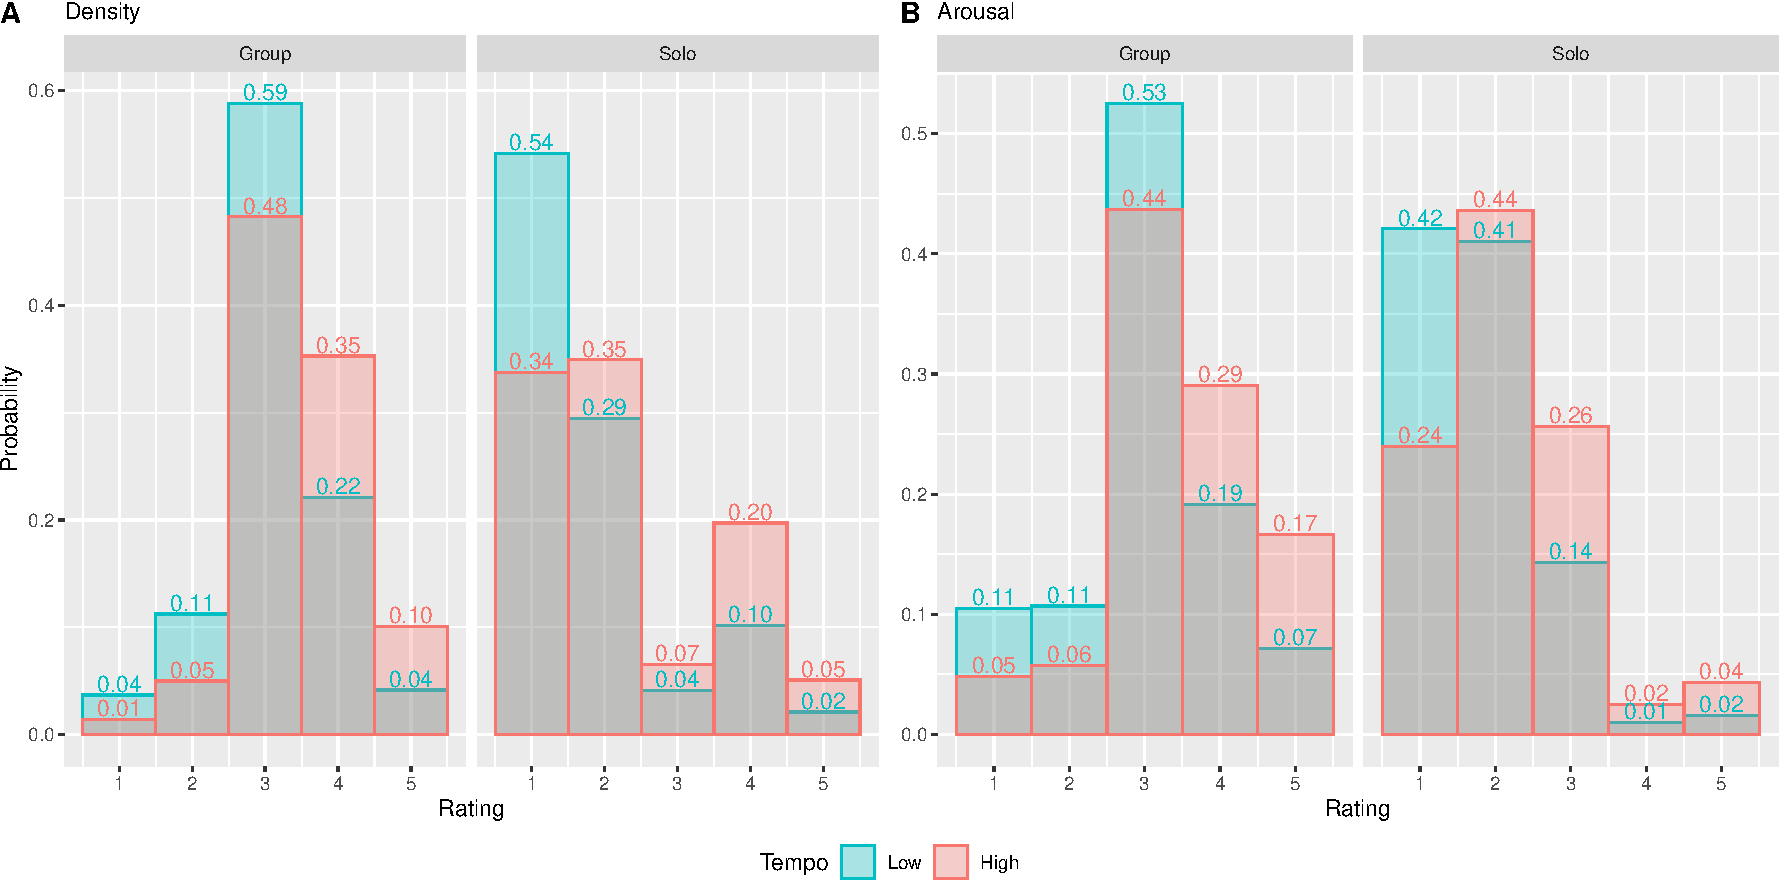
\includegraphics{Power_analysis_files/figure-latex/final-sim-1.pdf}
\caption{\label{fig:final-sim}Distribution of results from a conservative simulated distribution for ratings of both Density (\textbf{A}) and Arousal (\textbf{B}), by Instrumentation (Group, Solo), and Tempo (High, Low).}
\end{figure}

\hypertarget{comparisons-of-the-distribuition-of-results-between-pilot-and-simulated-data}{%
\subsection{Comparisons of the distribuition of results between pilot and simulated data}\label{comparisons-of-the-distribuition-of-results-between-pilot-and-simulated-data}}

\begin{Shaded}
\begin{Highlighting}[]
\NormalTok{p4 }\OtherTok{\textless{}{-}} \FunctionTok{ggarrange}\NormalTok{(}\FunctionTok{ggarrange}\NormalTok{(p1a }\SpecialCharTok{+} \FunctionTok{labs}\NormalTok{(}\AttributeTok{title =} \StringTok{"Pilot data"}\NormalTok{), }
\NormalTok{                          p1b }\SpecialCharTok{+} \FunctionTok{labs}\NormalTok{(}\AttributeTok{title =} \StringTok{" "}\NormalTok{),}
                          \AttributeTok{legend =} \StringTok{"none"}\NormalTok{), }
                \FunctionTok{ggarrange}\NormalTok{(p2a }\SpecialCharTok{+} \FunctionTok{labs}\NormalTok{(}\AttributeTok{title =} \StringTok{"Simulation (pilot data replication)"}\NormalTok{), }
\NormalTok{                          p2b }\SpecialCharTok{+} \FunctionTok{labs}\NormalTok{(}\AttributeTok{title =} \StringTok{" "}\NormalTok{),}
                          \AttributeTok{legend =} \StringTok{"none"}\NormalTok{),}
                \FunctionTok{ggarrange}\NormalTok{(p3a }\SpecialCharTok{+} \FunctionTok{labs}\NormalTok{(}\AttributeTok{title =} \StringTok{"Final simulation (conservative effect)"}\NormalTok{), }
\NormalTok{                          p3b }\SpecialCharTok{+} \FunctionTok{labs}\NormalTok{(}\AttributeTok{title =} \StringTok{" "}\NormalTok{),}
                          \AttributeTok{common.legend =} \ConstantTok{TRUE}\NormalTok{, }\AttributeTok{legend =} \StringTok{"bottom"}\NormalTok{),}
                \AttributeTok{common.legend =} \ConstantTok{TRUE}\NormalTok{,}
                \AttributeTok{labels =} \StringTok{"AUTO"}\NormalTok{,}
                \AttributeTok{nrow =} \DecValTok{3}\NormalTok{,}
                \AttributeTok{heights =} \FunctionTok{c}\NormalTok{(}\DecValTok{1}\NormalTok{,}\DecValTok{1}\NormalTok{,}\FloatTok{1.1}\NormalTok{))}
\NormalTok{p4}
\end{Highlighting}
\end{Shaded}

\begin{figure}
\centering
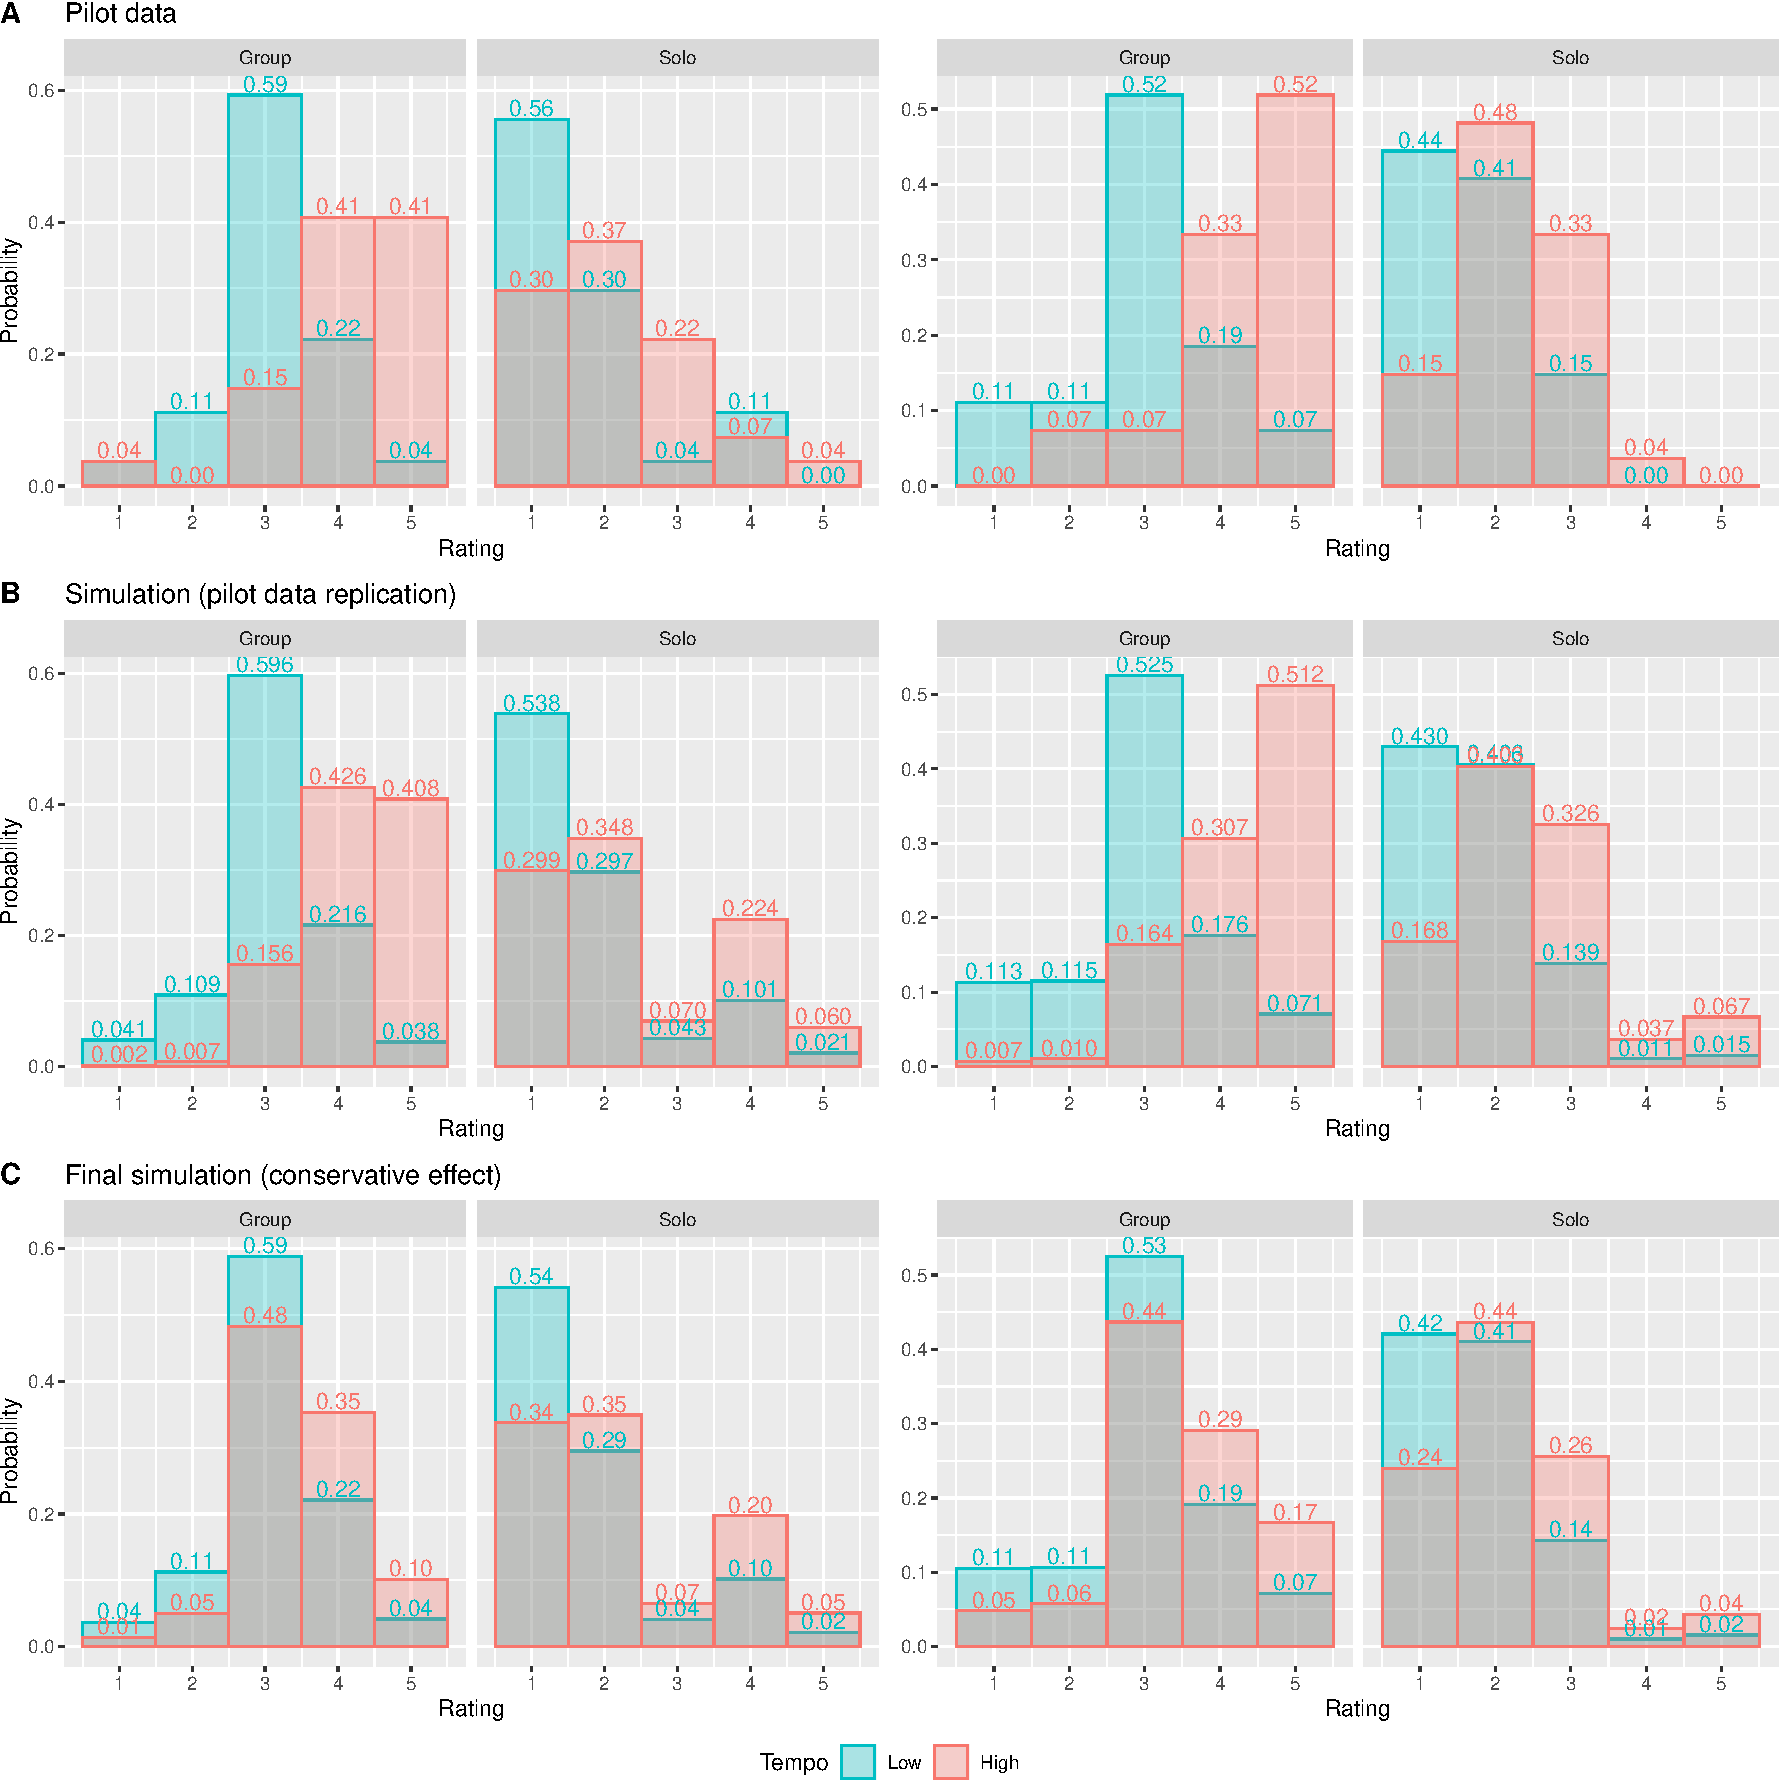
\includegraphics{Power_analysis_files/figure-latex/unnamed-chunk-12-1.pdf}
\caption{\label{fig:unnamed-chunk-12}Distribution of results of ratings of both Density and Arousal (\textbf{B}), by Instrumentation (Group, Solo), and Tempo (High, Low). \textbf{A} pilot data; \textbf{B} simulation replicating pilot data distribution; \textbf{C} simulation with a more conservative effect.}
\end{figure}

\hypertarget{power-section}{%
\section{Power analysis}\label{power-section}}

Using the final, simulated population (\emph{N} = 10,000 participants, with 6 paired observations per participant), we conducted a simulation-based power analysis. To do this, we first defined the desired number of simulations, the sample size (per country) of each simulation, and the \(\alpha\) value (significance level) for all statistical tests:

\begin{Shaded}
\begin{Highlighting}[]
\CommentTok{\# Number of simulations to run}
\NormalTok{num\_sims.clmm }\OtherTok{=} \DecValTok{1000} 

\CommentTok{\# Sample size for each simulation (number of participants per country)}
\NormalTok{sample\_size.clmm }\OtherTok{=} \DecValTok{24} 

\CommentTok{\# Significance level}
\NormalTok{alpha.clmm }\OtherTok{=} \FloatTok{0.05}
\end{Highlighting}
\end{Shaded}

Then, models were fitted from the defined 1,000 random samples extracted from the simulated population.

From each sample, two Cumulative Link Mixed Models (CLMM) were fitted \autocite[see e.g.,][]{taylorRatingNormsShould2022}: one for Density ratings, and one for arousal ratings. All models were fitted with the following call, simply changing the dependent variable (DV): \texttt{clmm(DV\ \textasciitilde{}\ Tempo\ *\ Solo.group\ *\ Participant.country\ *\ Music.country\ +\ (1\ +\ Tempo\ \textbar{}\ Participant)}.

This is, all models had the same structure, which included the main effects and all possible interactions between Tempo (Low, High), Instrumentation (Group, Solo), Participant country (Iran, Canada, Japan), and Music country (Iran, Canada, Japan) as fixed effects, as well as random intercepts and random slopes between Tempo conditions for each participant.

For each random sample, we adjusted the number of participants per country (in this case, \emph{n} = 24) to achieve the target statistical power of at least \(1 - \beta = 0.95\) for both the Density and Arousal models, for the contrast between Tempo levels (i.e., averaged over the levels of instrumentation, participant country and music country).

\hypertarget{select-random-samples}{%
\subsection{Select random samples}\label{select-random-samples}}

\begin{Shaded}
\begin{Highlighting}[]
\CommentTok{\# Get participant IDs}
\NormalTok{part }\OtherTok{\textless{}{-}}\NormalTok{ dat.sim  }\SpecialCharTok{|\textgreater{}} 
  \FunctionTok{group\_by}\NormalTok{(Participant.country) }\SpecialCharTok{|\textgreater{}}
  \FunctionTok{distinct}\NormalTok{(Participant) }\SpecialCharTok{|\textgreater{}}
  \FunctionTok{ungroup}\NormalTok{()}

\CommentTok{\# Select samples of random participants }
\NormalTok{samples.clmm }\OtherTok{\textless{}{-}} \FunctionTok{map\_dfr}\NormalTok{(}\FunctionTok{seq\_len}\NormalTok{(num\_sims.clmm), }\SpecialCharTok{\textasciitilde{}}\NormalTok{part }\SpecialCharTok{|\textgreater{}}
                        \FunctionTok{sample\_n}\NormalTok{(sample\_size.clmm) }\SpecialCharTok{|\textgreater{}}
                        \FunctionTok{mutate}\NormalTok{(}\AttributeTok{sample.clmm =} \FunctionTok{as.factor}\NormalTok{(.x)))}

\CommentTok{\# Final data base of data for each participant selected for each sample}
\NormalTok{samples.clmm.long }\OtherTok{\textless{}{-}} \FunctionTok{left\_join}\NormalTok{(samples.clmm, dat.sim, }\AttributeTok{by =} \FunctionTok{c}\NormalTok{(}\StringTok{"Participant"}\NormalTok{, }
                                                             \StringTok{"Participant.country"}\NormalTok{),}
                                \AttributeTok{relationship =} \StringTok{"many{-}to{-}many"}\NormalTok{) }\SpecialCharTok{|\textgreater{}}
  \FunctionTok{mutate}\NormalTok{(}\AttributeTok{Density.tempo =} \FunctionTok{as.factor}\NormalTok{(Density.tempo)) }\SpecialCharTok{|\textgreater{}}
  \FunctionTok{mutate}\NormalTok{(}\AttributeTok{Arousal.tempo =} \FunctionTok{as.factor}\NormalTok{(Arousal.tempo)) }\SpecialCharTok{|\textgreater{}}
  \FunctionTok{mutate}\NormalTok{(}\AttributeTok{Tempo =} \FunctionTok{as.factor}\NormalTok{(Tempo))}
\end{Highlighting}
\end{Shaded}

\hypertarget{visual-density-power-analysis}{%
\subsection{Visual density power analysis}\label{visual-density-power-analysis}}

Please be aware that this part of the simulation can take many ours (or even days) to run.

\begin{Shaded}
\begin{Highlighting}[]
\CommentTok{\# Create empty data frame}
\NormalTok{clmm.comps.den }\OtherTok{\textless{}{-}} \FunctionTok{data.frame}\NormalTok{(}\AttributeTok{Sample =} \DecValTok{1}\SpecialCharTok{:}\NormalTok{num\_sims.clmm)}

\CommentTok{\# Loop to fit a model for each random sample and extract the p{-}value of the Tempo contrasts}
\ControlFlowTok{for}\NormalTok{ (i }\ControlFlowTok{in} \DecValTok{1}\SpecialCharTok{:}\NormalTok{num\_sims.clmm)\{}
\NormalTok{  samp }\OtherTok{\textless{}{-}}\NormalTok{ samples.clmm.long }\SpecialCharTok{|\textgreater{}}
    \FunctionTok{filter}\NormalTok{(sample.clmm }\SpecialCharTok{==}\NormalTok{ i)}
  \FunctionTok{tryCatch}\NormalTok{(mod }\OtherTok{\textless{}{-}} \FunctionTok{clmm}\NormalTok{(Density.tempo }\SpecialCharTok{\textasciitilde{}} 
\NormalTok{                         Tempo }\SpecialCharTok{*}\NormalTok{ Solo.group }\SpecialCharTok{*}\NormalTok{ Participant.country }\SpecialCharTok{*}\NormalTok{ Music.country }\SpecialCharTok{+} 
\NormalTok{                         (}\DecValTok{1} \SpecialCharTok{+}\NormalTok{ Tempo }\SpecialCharTok{|}\NormalTok{ Participant), }\AttributeTok{data =}\NormalTok{ samp),}
           \AttributeTok{error =} \ControlFlowTok{function}\NormalTok{(e) \{\})}
  \FunctionTok{tryCatch}\NormalTok{(comp }\OtherTok{\textless{}{-}} \FunctionTok{emmeans}\NormalTok{(mod, pairwise}\SpecialCharTok{\textasciitilde{}}\NormalTok{Tempo),}
           \AttributeTok{error =} \ControlFlowTok{function}\NormalTok{(e) \{\})}
\NormalTok{  clmm.comps.den}\SpecialCharTok{$}\NormalTok{p[i] }\OtherTok{\textless{}{-}} \FunctionTok{round}\NormalTok{(}\FunctionTok{data.frame}\NormalTok{(comp}\SpecialCharTok{$}\NormalTok{contrast)}\SpecialCharTok{$}\NormalTok{p.value, }\DecValTok{3}\NormalTok{)}
\NormalTok{  clmm.comps.den}\SpecialCharTok{$}\StringTok{\textasciigrave{}}\AttributeTok{Statistical signicance}\StringTok{\textasciigrave{}}\NormalTok{[i] }\OtherTok{\textless{}{-}} \FunctionTok{ifelse}\NormalTok{(clmm.comps.den}\SpecialCharTok{$}\NormalTok{p[i] }\SpecialCharTok{\textless{}=}\NormalTok{ alpha.clmm, }
                                                       \StringTok{"Significant"}\NormalTok{, }\StringTok{"Non{-}significant"}\NormalTok{)}
\NormalTok{\}}

\CommentTok{\# Calculate power (proportion of simulations in which the Tempo contrast was significant)}
\NormalTok{power.clmm.den }\OtherTok{\textless{}{-}} \FunctionTok{sum}\NormalTok{(clmm.comps.den}\SpecialCharTok{$}\StringTok{\textasciigrave{}}\AttributeTok{Statistical signicance}\StringTok{\textasciigrave{}} \SpecialCharTok{==} \StringTok{"Significant"}\NormalTok{)}\SpecialCharTok{/}\NormalTok{num\_sims.clmm}
\end{Highlighting}
\end{Shaded}

\hypertarget{arousal-power-analysis}{%
\subsection{Arousal power analysis}\label{arousal-power-analysis}}

Again, please keep in mind that this part of the simulation can take many ours (or even days) to run.

\begin{Shaded}
\begin{Highlighting}[]
\CommentTok{\# Create empty data frame}
\NormalTok{clmm.comps.aro }\OtherTok{\textless{}{-}} \FunctionTok{data.frame}\NormalTok{(}\AttributeTok{Sample =} \DecValTok{1}\SpecialCharTok{:}\NormalTok{num\_sims.clmm)}

\CommentTok{\# Loop to fit a model for each random sample and extract the p{-}value of the Tempo contrasts}
\ControlFlowTok{for}\NormalTok{ (i }\ControlFlowTok{in} \DecValTok{1}\SpecialCharTok{:}\NormalTok{num\_sims.clmm)\{}
\NormalTok{  samp }\OtherTok{\textless{}{-}}\NormalTok{ samples.clmm.long }\SpecialCharTok{|\textgreater{}}
    \FunctionTok{filter}\NormalTok{(sample.clmm }\SpecialCharTok{==}\NormalTok{ i)}
  \FunctionTok{tryCatch}\NormalTok{(mod }\OtherTok{\textless{}{-}} \FunctionTok{clmm}\NormalTok{(Arousal.tempo }\SpecialCharTok{\textasciitilde{}} 
\NormalTok{                         Tempo }\SpecialCharTok{*}\NormalTok{ Solo.group }\SpecialCharTok{*}\NormalTok{ Participant.country }\SpecialCharTok{*}\NormalTok{ Music.country }\SpecialCharTok{+} 
\NormalTok{                         (}\DecValTok{1} \SpecialCharTok{+}\NormalTok{ Tempo }\SpecialCharTok{|}\NormalTok{ Participant), }\AttributeTok{data =}\NormalTok{ samp),}
           \AttributeTok{error =} \ControlFlowTok{function}\NormalTok{(e) \{\})}
  \FunctionTok{tryCatch}\NormalTok{(comp }\OtherTok{\textless{}{-}} \FunctionTok{emmeans}\NormalTok{(mod, pairwise}\SpecialCharTok{\textasciitilde{}}\NormalTok{Tempo),}
           \AttributeTok{error =} \ControlFlowTok{function}\NormalTok{(e) \{\})}
\NormalTok{  clmm.comps.aro}\SpecialCharTok{$}\NormalTok{p[i] }\OtherTok{\textless{}{-}} \FunctionTok{round}\NormalTok{(}\FunctionTok{data.frame}\NormalTok{(comp}\SpecialCharTok{$}\NormalTok{contrast)}\SpecialCharTok{$}\NormalTok{p.value, }\DecValTok{3}\NormalTok{)}
\NormalTok{  clmm.comps.aro}\SpecialCharTok{$}\StringTok{\textasciigrave{}}\AttributeTok{Statistical signicance}\StringTok{\textasciigrave{}}\NormalTok{[i] }\OtherTok{\textless{}{-}} \FunctionTok{ifelse}\NormalTok{(clmm.comps.aro}\SpecialCharTok{$}\NormalTok{p[i] }\SpecialCharTok{\textless{}=}\NormalTok{ alpha.clmm, }
                                                       \StringTok{"Significant"}\NormalTok{, }\StringTok{"Non{-}significant"}\NormalTok{)}
\NormalTok{\}}

\CommentTok{\# Calculate power (proportion of simulations in which the Tempo contrast was significant)}
\NormalTok{power.clmm.aro }\OtherTok{\textless{}{-}} \FunctionTok{sum}\NormalTok{(clmm.comps.aro}\SpecialCharTok{$}\StringTok{\textasciigrave{}}\AttributeTok{Statistical signicance}\StringTok{\textasciigrave{}} \SpecialCharTok{==} \StringTok{"Significant"}\NormalTok{)}\SpecialCharTok{/}\NormalTok{num\_sims.clmm}
\end{Highlighting}
\end{Shaded}

\hypertarget{achieved-power-plot}{%
\subsection{Achieved power plot}\label{achieved-power-plot}}

\begin{Shaded}
\begin{Highlighting}[]
\NormalTok{p5a }\OtherTok{\textless{}{-}} \FunctionTok{ggplot}\NormalTok{(clmm.comps.den, }\FunctionTok{aes}\NormalTok{(}\AttributeTok{x =}\NormalTok{ p, }\AttributeTok{fill =} \StringTok{\textasciigrave{}}\AttributeTok{Statistical signicance}\StringTok{\textasciigrave{}}\NormalTok{)) }\SpecialCharTok{+}
  \FunctionTok{scale\_fill\_hue}\NormalTok{(}\AttributeTok{direction =} \SpecialCharTok{{-}}\DecValTok{1}\NormalTok{) }\SpecialCharTok{+}
  \FunctionTok{geom\_histogram}\NormalTok{(}\AttributeTok{bins =} \DecValTok{1}\SpecialCharTok{/}\NormalTok{alpha.clmm, }\AttributeTok{breaks =} \FunctionTok{seq}\NormalTok{(}\DecValTok{0}\NormalTok{, }\DecValTok{1}\NormalTok{, alpha.clmm)) }\SpecialCharTok{+}
  \FunctionTok{labs}\NormalTok{(}\AttributeTok{y =} \StringTok{"Count"}\NormalTok{, }\AttributeTok{x =} \StringTok{"p{-}value"}\NormalTok{, }\AttributeTok{title =} \StringTok{"Density"}\NormalTok{) }\SpecialCharTok{+}
  \FunctionTok{annotate}\NormalTok{(}\StringTok{"text"}\NormalTok{, }\AttributeTok{x =} \FloatTok{0.5}\NormalTok{, }
           \AttributeTok{y =} \FunctionTok{sum}\NormalTok{(clmm.comps.den}\SpecialCharTok{$}\StringTok{\textasciigrave{}}\AttributeTok{Statistical signicance}\StringTok{\textasciigrave{}} \SpecialCharTok{==} \StringTok{"Significant"}\NormalTok{) }\SpecialCharTok{*} \FloatTok{0.9}\NormalTok{,}
           \AttributeTok{label =} \FunctionTok{paste0}\NormalTok{(}\StringTok{"Power = "}\NormalTok{, }\FunctionTok{round}\NormalTok{(power.clmm.den, }\DecValTok{3}\NormalTok{),}
                          \StringTok{"}\SpecialCharTok{\textbackslash{}n}\StringTok{Sample size = "}\NormalTok{, sample\_size.clmm,}
                          \StringTok{" participants per country}\SpecialCharTok{\textbackslash{}n}\StringTok{(6 paired responses per participant)"}\NormalTok{))}

\NormalTok{p5b }\OtherTok{\textless{}{-}} \FunctionTok{ggplot}\NormalTok{(clmm.comps.aro, }\FunctionTok{aes}\NormalTok{(}\AttributeTok{x =}\NormalTok{ p, }\AttributeTok{fill =} \StringTok{\textasciigrave{}}\AttributeTok{Statistical signicance}\StringTok{\textasciigrave{}}\NormalTok{)) }\SpecialCharTok{+}
  \FunctionTok{scale\_fill\_hue}\NormalTok{(}\AttributeTok{direction =} \SpecialCharTok{{-}}\DecValTok{1}\NormalTok{) }\SpecialCharTok{+}
  \FunctionTok{geom\_histogram}\NormalTok{(}\AttributeTok{bins =} \DecValTok{1}\SpecialCharTok{/}\NormalTok{alpha.clmm, }\AttributeTok{breaks =} \FunctionTok{seq}\NormalTok{(}\DecValTok{0}\NormalTok{, }\DecValTok{1}\NormalTok{, alpha.clmm)) }\SpecialCharTok{+}
  \FunctionTok{labs}\NormalTok{(}\AttributeTok{y =} \StringTok{"Count"}\NormalTok{, }\AttributeTok{x =} \StringTok{"p{-}value"}\NormalTok{, }\AttributeTok{title =} \StringTok{"Arousal"}\NormalTok{) }\SpecialCharTok{+}
  \FunctionTok{annotate}\NormalTok{(}\StringTok{"text"}\NormalTok{, }\AttributeTok{x =} \FloatTok{0.5}\NormalTok{, }
           \AttributeTok{y =} \FunctionTok{sum}\NormalTok{(clmm.comps.aro}\SpecialCharTok{$}\StringTok{\textasciigrave{}}\AttributeTok{Statistical signicance}\StringTok{\textasciigrave{}} \SpecialCharTok{==} \StringTok{"Significant"}\NormalTok{) }\SpecialCharTok{*} \FloatTok{0.9}\NormalTok{, }
           \AttributeTok{label =} \FunctionTok{paste0}\NormalTok{(}\StringTok{"Power = "}\NormalTok{, }\FunctionTok{round}\NormalTok{(power.clmm.aro, }\DecValTok{3}\NormalTok{), }
                          \StringTok{"}\SpecialCharTok{\textbackslash{}n}\StringTok{Sample size = "}\NormalTok{, sample\_size.clmm, }
                          \StringTok{" participants per country}\SpecialCharTok{\textbackslash{}n}\StringTok{(6 paired responses per participant)"}\NormalTok{))}

\NormalTok{p5 }\OtherTok{\textless{}{-}} \FunctionTok{ggarrange}\NormalTok{(p5a, p5b,}
                \AttributeTok{common.legend =} \ConstantTok{TRUE}\NormalTok{,}
                \AttributeTok{legend =} \StringTok{"bottom"}\NormalTok{,}
                \AttributeTok{labels =} \StringTok{"AUTO"}\NormalTok{)}
\NormalTok{p5}
\end{Highlighting}
\end{Shaded}

\begin{figure}
\centering
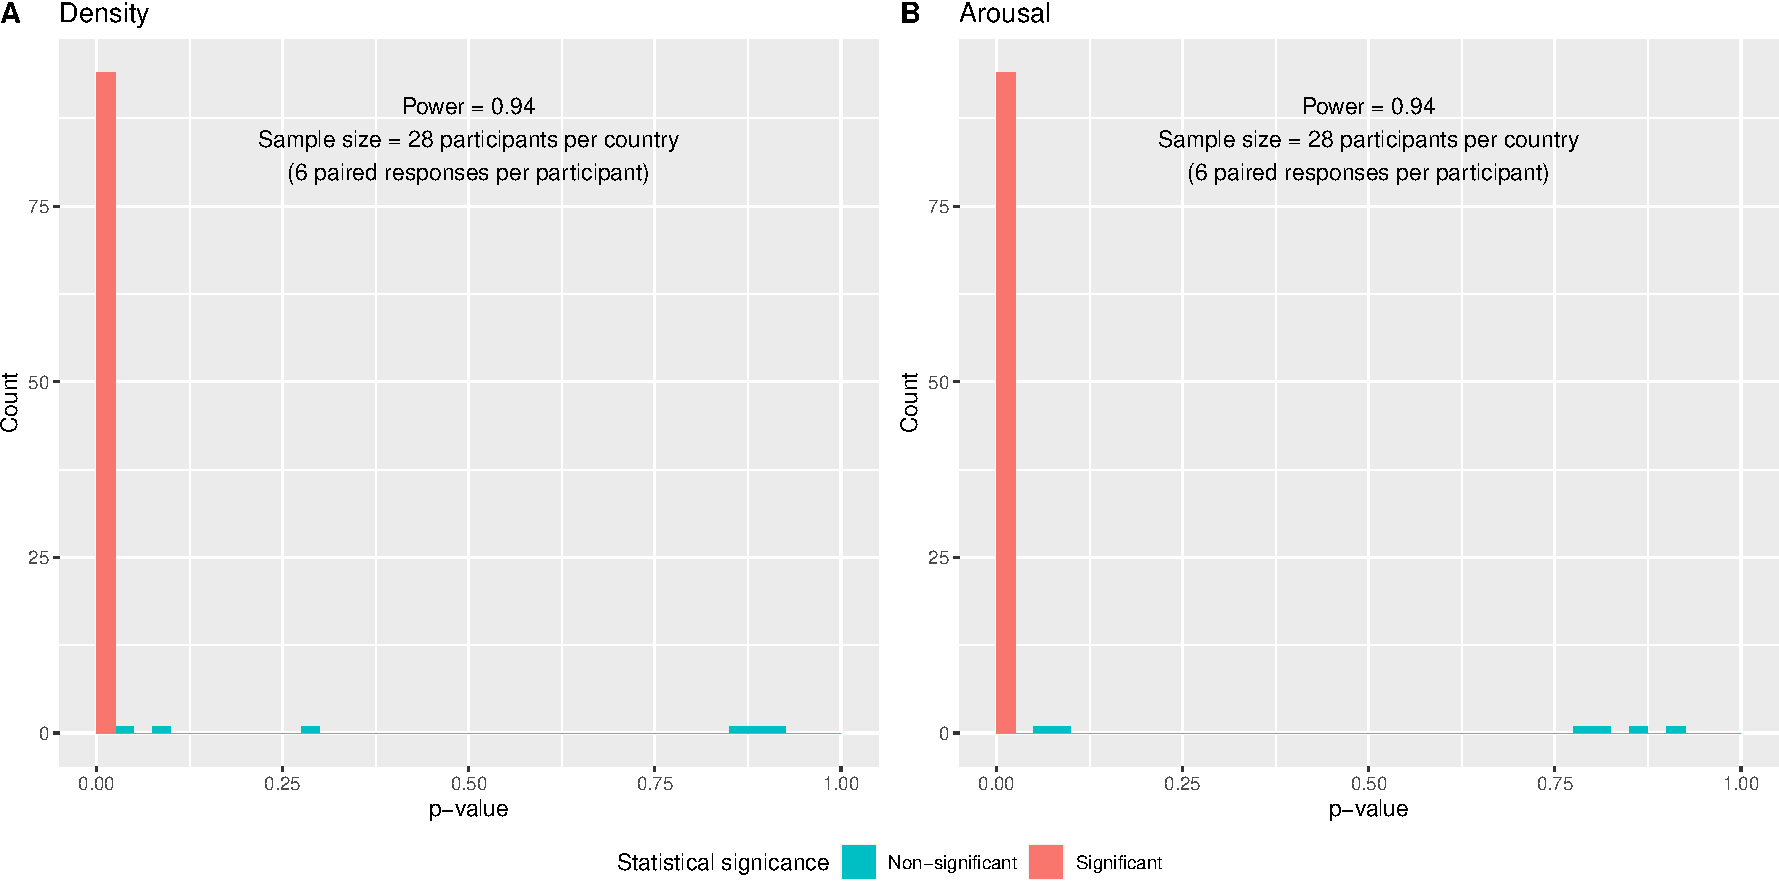
\includegraphics{Power_analysis_files/figure-latex/unnamed-chunk-15-1.pdf}
\caption{\label{fig:unnamed-chunk-15}Histogram of \emph{p}-values for the contrasts between Tempo conditions (Low, High) for all simulations. The estatistical power is the proportion of significant results. Significant results are in red.}
\end{figure}

\hypertarget{example-data}{%
\section{Analysis script with example data}\label{example-data}}

Here, using a randomly selected sample, we fit one model as if it was the data collected from the experiment. This is not only to make sure that the data are sufficient and the structure is adequate to fit the model, but to plan in advance all the code.

\begin{Shaded}
\begin{Highlighting}[]
\FunctionTok{set.seed}\NormalTok{(}\DecValTok{1}\NormalTok{)}
\CommentTok{\# Select a random sample}
\NormalTok{ex.data }\OtherTok{\textless{}{-}}\NormalTok{ samples.clmm.long  }\SpecialCharTok{|\textgreater{}} 
  \FunctionTok{filter}\NormalTok{(sample.clmm }\SpecialCharTok{==} \FunctionTok{sample}\NormalTok{(}\DecValTok{1}\SpecialCharTok{:}\NormalTok{num\_sims.clmm, }\DecValTok{1}\NormalTok{, }\AttributeTok{replace =} \ConstantTok{TRUE}\NormalTok{)) }\SpecialCharTok{|\textgreater{}} 
  \FunctionTok{mutate\_if}\NormalTok{(is.character,as.factor)}
\end{Highlighting}
\end{Shaded}

Because only the effect of Tempo was predicted and simulated \emph{a-priori}, all other effects and interactions are completely random.

\begin{Shaded}
\begin{Highlighting}[]
\NormalTok{p6a }\OtherTok{\textless{}{-}} \FunctionTok{ggplot}\NormalTok{(ex.data, }\FunctionTok{aes}\NormalTok{(}\AttributeTok{x =}\NormalTok{ Tempo, }\AttributeTok{y =}\NormalTok{ Density.tempo, }
                           \AttributeTok{color =}\NormalTok{ Participant.country, }\AttributeTok{shape =}\NormalTok{ Music.country)) }\SpecialCharTok{+}
  \FunctionTok{geom\_violin}\NormalTok{(}\FunctionTok{aes}\NormalTok{(}\AttributeTok{group =}\NormalTok{ Tempo), }\AttributeTok{draw\_quantiles =} \FloatTok{0.5}\NormalTok{) }\SpecialCharTok{+}
  \FunctionTok{geom\_point}\NormalTok{(}\AttributeTok{position =} \FunctionTok{position\_dodge}\NormalTok{(}\FloatTok{0.3}\NormalTok{), }\AttributeTok{size =} \DecValTok{3}\NormalTok{) }\SpecialCharTok{+}
  \FunctionTok{geom\_line}\NormalTok{(}\FunctionTok{aes}\NormalTok{(}\AttributeTok{group =} \FunctionTok{factor}\NormalTok{(groupid)), }
            \AttributeTok{linewidth =} \FloatTok{0.5}\NormalTok{, }\AttributeTok{linetype =} \StringTok{"dashed"}\NormalTok{, }\AttributeTok{position =} \FunctionTok{position\_dodge}\NormalTok{(}\FloatTok{0.3}\NormalTok{), }\AttributeTok{alpha =} \FloatTok{0.5}\NormalTok{) }\SpecialCharTok{+}
  \FunctionTok{labs}\NormalTok{(}\AttributeTok{y=} \StringTok{"Density"}\NormalTok{, }\AttributeTok{x =} \StringTok{"Tempo"}\NormalTok{, }\AttributeTok{title =} \StringTok{"Density"}\NormalTok{) }\SpecialCharTok{+}
  \FunctionTok{scale\_x\_discrete}\NormalTok{(}\AttributeTok{limits =} \FunctionTok{c}\NormalTok{(}\StringTok{"Low"}\NormalTok{, }\StringTok{"High"}\NormalTok{)) }\SpecialCharTok{+} 
  \FunctionTok{scale\_size\_discrete}\NormalTok{(}\AttributeTok{breaks =} \FunctionTok{c}\NormalTok{(}\StringTok{"Solo"}\NormalTok{, }\StringTok{"Group"}\NormalTok{)) }\SpecialCharTok{+} 
  \FunctionTok{theme}\NormalTok{(}\AttributeTok{plot.title =} \FunctionTok{element\_text}\NormalTok{(}\AttributeTok{face =} \StringTok{"bold"}\NormalTok{, }\AttributeTok{hjust =} \FloatTok{0.5}\NormalTok{)) }\SpecialCharTok{+} 
  \FunctionTok{facet\_wrap}\NormalTok{(}\SpecialCharTok{\textasciitilde{}}\NormalTok{Solo.group)}

\NormalTok{p6b }\OtherTok{\textless{}{-}} \FunctionTok{ggplot}\NormalTok{(ex.data, }\FunctionTok{aes}\NormalTok{(}\AttributeTok{x =}\NormalTok{ Tempo, }\AttributeTok{y =}\NormalTok{ Arousal.tempo, }
                           \AttributeTok{color =}\NormalTok{ Participant.country, }\AttributeTok{shape =}\NormalTok{ Music.country)) }\SpecialCharTok{+}
   \FunctionTok{geom\_violin}\NormalTok{(}\FunctionTok{aes}\NormalTok{(}\AttributeTok{group =}\NormalTok{ Tempo), }\AttributeTok{draw\_quantiles =} \FloatTok{0.5}\NormalTok{) }\SpecialCharTok{+}
  \FunctionTok{geom\_point}\NormalTok{(}\AttributeTok{position =} \FunctionTok{position\_dodge}\NormalTok{(}\FloatTok{0.3}\NormalTok{), }\AttributeTok{size =} \DecValTok{3}\NormalTok{) }\SpecialCharTok{+}
  \FunctionTok{geom\_line}\NormalTok{(}\FunctionTok{aes}\NormalTok{(}\AttributeTok{group =} \FunctionTok{factor}\NormalTok{(groupid)), }
            \AttributeTok{linewidth =} \FloatTok{0.5}\NormalTok{, }\AttributeTok{linetype =} \StringTok{"dashed"}\NormalTok{, }\AttributeTok{position =} \FunctionTok{position\_dodge}\NormalTok{(}\FloatTok{0.3}\NormalTok{), }\AttributeTok{alpha =} \FloatTok{0.5}\NormalTok{) }\SpecialCharTok{+}
  \FunctionTok{labs}\NormalTok{(}\AttributeTok{y=} \StringTok{"Arousal"}\NormalTok{, }\AttributeTok{x =} \StringTok{"Tempo"}\NormalTok{, }\AttributeTok{title =} \StringTok{"Arousal"}\NormalTok{) }\SpecialCharTok{+}
  \FunctionTok{scale\_x\_discrete}\NormalTok{(}\AttributeTok{limits =} \FunctionTok{c}\NormalTok{(}\StringTok{"Low"}\NormalTok{, }\StringTok{"High"}\NormalTok{)) }\SpecialCharTok{+} 
  \FunctionTok{scale\_size\_discrete}\NormalTok{(}\AttributeTok{breaks =} \FunctionTok{c}\NormalTok{(}\StringTok{"Solo"}\NormalTok{, }\StringTok{"Group"}\NormalTok{)) }\SpecialCharTok{+} 
  \FunctionTok{theme}\NormalTok{(}\AttributeTok{plot.title =} \FunctionTok{element\_text}\NormalTok{(}\AttributeTok{face =} \StringTok{"bold"}\NormalTok{, }\AttributeTok{hjust =} \FloatTok{0.5}\NormalTok{)) }\SpecialCharTok{+} 
  \FunctionTok{facet\_wrap}\NormalTok{(}\SpecialCharTok{\textasciitilde{}}\NormalTok{Solo.group)}

\NormalTok{p6 }\OtherTok{\textless{}{-}} \FunctionTok{ggarrange}\NormalTok{(p6a, p6b,}
                \AttributeTok{common.legend =} \ConstantTok{TRUE}\NormalTok{,}
                \AttributeTok{legend =} \StringTok{"bottom"}\NormalTok{)}
\NormalTok{p6}
\end{Highlighting}
\end{Shaded}

\begin{figure}
\centering
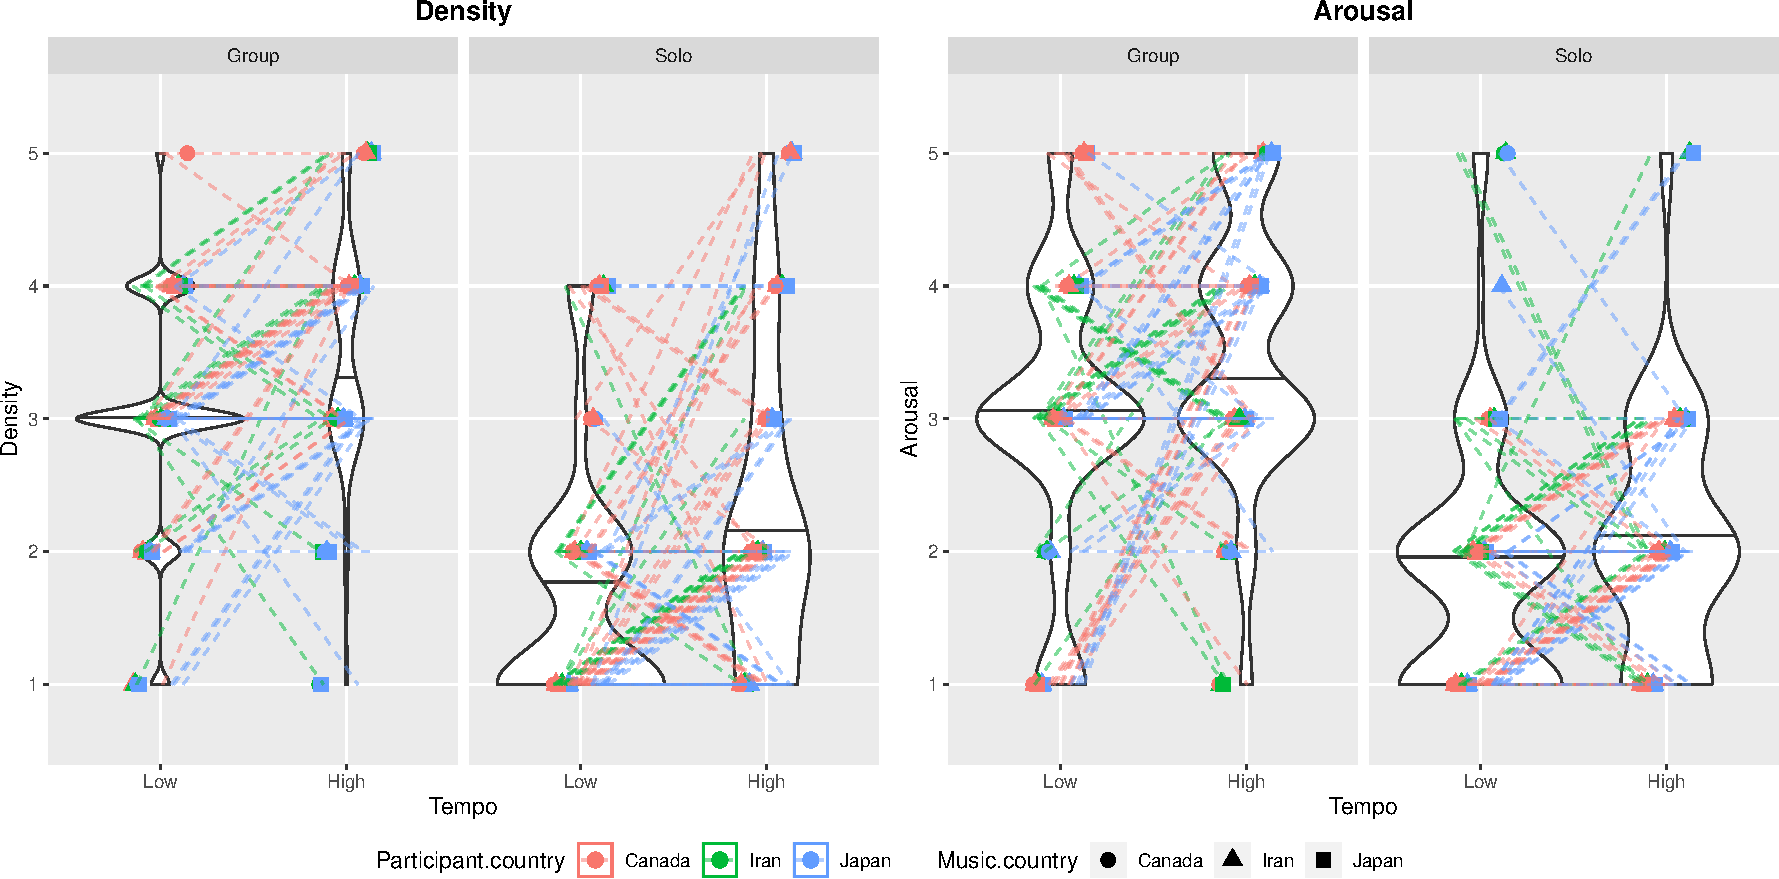
\includegraphics{Power_analysis_files/figure-latex/unnamed-chunk-17-1.pdf}
\caption{\label{fig:unnamed-chunk-17}Data for Density and Arousal ratings from a ramdomly selected, simulated sample. Dashed linesrepresent the within-subject effect of the Tempo manipulation.}
\end{figure}

We fitted the models with the same structure, simply changing the dependent variable (DV): \texttt{clmm(DV\ \textasciitilde{}\ Tempo\ *\ Solo.group\ *\ Participant.country\ *\ Music.country\ +\ (1\ +\ Tempo\ \textbar{}\ Participant)}. To obtain \emph{p}-values that represent main effects and interactions in an ANOVA-type manner (i.e.~the intercept is the grand mean of all cells, and estimates are differences between each category mean and the mean of all categories), we used \emph{sum-to-zero} contrasts\footnote{We did not do this for the models fitted for the power analysis, as it would not change the contrasts between Tempo conditions, but it is useful to display the full model results as we used \texttt{summary} (regression-type tables of estimates) instead on ANOVA-type tables (which are not available for models of \texttt{clmm} class).} \autocites[see e.g.,][]{kaufmanContrastCodingLeast1974,keppelDataAnalysisResearch1989}.

In all cases, results are for main effects and all possible interactions between Tempo (Low, High), Instrumentation (Group, Solo), Participant country (Iran, Canada, Japan), and Music country (Iran, Canada, Japan) as fixed effects, as well as random intercepts and random slopes between Tempo conditions for each participant. \emph{High} was used as reference category for Tempo, and \emph{Japan} for both participant and music country. Contrasted levels are in square brackets. Significant effects are in bold.

As pointed out in a comment by \textcite{532079}, author of the \texttt{emmeans} package \autocite*{emmeanscit}, it is crucial to consider that ordinal models rely on estimates of a dependent variable (\emph{y}) following a logistic distribution. However, \emph{y} itself cannot be directly observed; rather, only the interval in which it lies is observable. Consequently, \emph{y} is an unobserved latent variable. Thus, in order to interpret the estimates, the model also calculates the thresholds (cut points) for the ordinal levels of the dependent variable.

\hypertarget{visual-density-example-model}{%
\subsection{Visual density example model}\label{visual-density-example-model}}

\begin{Shaded}
\begin{Highlighting}[]
\CommentTok{\# Fit Density model}
\FunctionTok{options}\NormalTok{(}\AttributeTok{contrasts =} \FunctionTok{c}\NormalTok{(}\StringTok{"contr.sum"}\NormalTok{,}\StringTok{"contr.poly"}\NormalTok{))}
\NormalTok{model.den }\OtherTok{\textless{}{-}} \FunctionTok{clmm}\NormalTok{(Density.tempo }\SpecialCharTok{\textasciitilde{}}\NormalTok{ Tempo }\SpecialCharTok{*}\NormalTok{ Solo.group }\SpecialCharTok{*}\NormalTok{ Participant.country }\SpecialCharTok{*}\NormalTok{ Music.country }\SpecialCharTok{+} 
\NormalTok{                    (}\DecValTok{1} \SpecialCharTok{+}\NormalTok{ Tempo }\SpecialCharTok{|}\NormalTok{ Participant),}
                  \AttributeTok{data =}\NormalTok{ ex.data)}

\CommentTok{\# Summary table}
\FunctionTok{summary.sig}\NormalTok{(model.den, }\StringTok{"Visual density ratings model summary"}\NormalTok{)}
\end{Highlighting}
\end{Shaded}

\begin{table}[H]

\caption{\label{tab:mod-ex-den}Visual density ratings model summary}
\centering
\resizebox{\linewidth}{!}{
\begin{tabular}[t]{lcccc}
\toprule
Effects & Estimate & Std. Error & $z$ & $p$\\
\midrule
\addlinespace[0.3em]
\multicolumn{5}{l}{\textbf{Thresholds}}\\
\hline
\hspace{1em}1|2 & -1.87 & 0.22 & -8.39 & \textbf{< 0.0001}\\
\hspace{1em}2|3 & -0.36 & 0.19 & -1.88 & 0.06\\
\hspace{1em}3|4 & 1.72 & 0.21 & 8.38 & \textbf{< 0.0001}\\
\hspace{1em}4|5 & 3.77 & 0.31 & 12.32 & \textbf{< 0.0001}\\
\addlinespace[0.3em]
\hline
\multicolumn{5}{l}{\textbf{Terms}}\\
\hline
\hspace{1em}Tempo [Low] & -0.48 & 0.13 & -3.80 & \textbf{< 0.001}\\
\hspace{1em}Instrumentation [Group] & 1.53 & 0.15 & 10.20 & \textbf{< 0.0001}\\
\hspace{1em}Participant country [Canada] & 0.51 & 0.20 & 2.57 & \textbf{0.0101}\\
\hspace{1em}Participant country [Iran] & -0.39 & 0.22 & -1.72 & 0.08\\
\hspace{1em}Music country [Canada] & 0.00 & 0.17 & -0.02 & 0.98\\
\hspace{1em}Music country [Iran] & 0.19 & 0.17 & 1.14 & 0.25\\
\hspace{1em}Tempo [Low] × Instrumentation [Group] & 0.12 & 0.12 & 1.00 & 0.32\\
\hspace{1em}Tempo [Low] × Participant country [Canada] & 0.12 & 0.16 & 0.74 & 0.46\\
\hspace{1em}Tempo [Low] × Participant country [Iran] & -0.18 & 0.18 & -1.01 & 0.31\\
\hspace{1em}Instrumentation [Group] × Participant country [Canada] & -0.51 & 0.15 & -3.30 & \textbf{< 0.001}\\
\hspace{1em}Instrumentation [Group] × Participant country [Iran] & 0.04 & 0.18 & 0.24 & 0.81\\
\hspace{1em}Tempo [Low] × Music country [Canada] & 0.01 & 0.17 & 0.04 & 0.96\\
\hspace{1em}Tempo [Low] × Music country [Iran] & 0.04 & 0.17 & 0.26 & 0.8\\
\hspace{1em}Instrumentation [Group] × Music country [Canada] & 0.21 & 0.17 & 1.25 & 0.21\\
\hspace{1em}Instrumentation [Group] × Music country [Iran] & -0.25 & 0.17 & -1.51 & 0.13\\
\hspace{1em}Participant country [Canada] × Music country [Canada] & -0.25 & 0.21 & -1.17 & 0.24\\
\hspace{1em}Participant country [Iran] × Music country [Canada] & 0.29 & 0.24 & 1.19 & 0.24\\
\hspace{1em}Participant country [Canada] × Music country [Iran] & 0.36 & 0.22 & 1.66 & 0.1\\
\hspace{1em}Participant country [Iran] × Music country [Iran] & -0.44 & 0.25 & -1.78 & 0.08\\
\hspace{1em}Tempo [Low] × Instrumentation [Group] × Participant country [Canada] & 0.01 & 0.15 & 0.07 & 0.94\\
\hspace{1em}Tempo [Low] × Instrumentation [Group] × Participant country [Iran] & 0.34 & 0.18 & 1.96 & 0.05\\
\hspace{1em}Tempo [Low] × Instrumentation [Group] × Music country [Canada] & 0.05 & 0.17 & 0.33 & 0.74\\
\hspace{1em}Tempo [Low] × Instrumentation [Group] × Music country [Iran] & -0.08 & 0.17 & -0.46 & 0.65\\
\hspace{1em}Tempo [Low] × Participant country [Canada] × Music country [Canada] & -0.13 & 0.21 & -0.63 & 0.53\\
\hspace{1em}Tempo [Low] × Participant country [Iran] × Music country [Canada] & 0.24 & 0.24 & 0.99 & 0.32\\
\hspace{1em}Tempo [Low] × Participant country [Canada] × Music country [Iran] & -0.01 & 0.22 & -0.04 & 0.97\\
\hspace{1em}Tempo [Low] × Participant country [Iran] × Music country [Iran] & 0.20 & 0.25 & 0.82 & 0.41\\
\hspace{1em}Instrumentation [Group] × Participant country [Canada] × Music country [Canada] & 0.20 & 0.21 & 0.96 & 0.34\\
\hspace{1em}Instrumentation [Group] × Participant country [Iran] × Music country [Canada] & -0.42 & 0.24 & -1.73 & 0.08\\
\hspace{1em}Instrumentation [Group] × Participant country [Canada] × Music country [Iran] & -0.25 & 0.22 & -1.15 & 0.25\\
\hspace{1em}Instrumentation [Group] × Participant country [Iran] × Music country [Iran] & 0.26 & 0.25 & 1.05 & 0.29\\
\hspace{1em}Tempo [Low] × Instrumentation [Group] × Participant country [Canada] × Music country [Canada] & 0.02 & 0.21 & 0.10 & 0.92\\
\hspace{1em}Tempo [Low] × Instrumentation [Group] × Participant country [Iran] × Music country [Canada] & 0.19 & 0.24 & 0.80 & 0.43\\
\hspace{1em}Tempo [Low] × Instrumentation [Group] × Participant country [Canada] × Music country [Iran] & 0.12 & 0.22 & 0.57 & 0.57\\
\hspace{1em}Tempo [Low] × Instrumentation [Group] × Participant country [Iran] × Music country [Iran] & -0.11 & 0.25 & -0.46 & 0.65\\
\bottomrule
\end{tabular}}
\end{table}

\hypertarget{arousal-example-model}{%
\subsection{Arousal example model}\label{arousal-example-model}}

\begin{Shaded}
\begin{Highlighting}[]
\CommentTok{\# Fit Arousal model}
\FunctionTok{options}\NormalTok{(}\AttributeTok{contrasts =} \FunctionTok{c}\NormalTok{(}\StringTok{"contr.sum"}\NormalTok{,}\StringTok{"contr.poly"}\NormalTok{))}
\NormalTok{model.aro }\OtherTok{\textless{}{-}} \FunctionTok{clmm}\NormalTok{(Arousal.tempo }\SpecialCharTok{\textasciitilde{}}\NormalTok{ Tempo }\SpecialCharTok{*}\NormalTok{ Solo.group }\SpecialCharTok{*}\NormalTok{ Participant.country }\SpecialCharTok{*}\NormalTok{ Music.country }\SpecialCharTok{+} 
\NormalTok{                    (}\DecValTok{1} \SpecialCharTok{+}\NormalTok{ Tempo }\SpecialCharTok{|}\NormalTok{ Participant),}
                  \AttributeTok{data =}\NormalTok{ ex.data)}

\CommentTok{\# Summary table}
\FunctionTok{summary.sig}\NormalTok{(model.aro, }\StringTok{"Arousal ratings model summary"}\NormalTok{)}
\end{Highlighting}
\end{Shaded}

\begin{table}[H]

\caption{\label{tab:mod-ex-aro}Arousal ratings model summary}
\centering
\resizebox{\linewidth}{!}{
\begin{tabular}[t]{lcccc}
\toprule
Effects & Estimate & Std. Error & $z$ & $p$\\
\midrule
\addlinespace[0.3em]
\multicolumn{5}{l}{\textbf{Thresholds}}\\
\hline
\hspace{1em}1|2 & -2.02 & 0.20 & -9.88 & \textbf{< 0.0001}\\
\hspace{1em}2|3 & -0.27 & 0.17 & -1.63 & 0.1\\
\hspace{1em}3|4 & 2.08 & 0.21 & 9.80 & \textbf{< 0.0001}\\
\hspace{1em}4|5 & 3.46 & 0.29 & 12.03 & \textbf{< 0.0001}\\
\addlinespace[0.3em]
\hline
\multicolumn{5}{l}{\textbf{Terms}}\\
\hline
\hspace{1em}Tempo [Low] & -0.62 & 0.13 & -4.84 & \textbf{< 0.0001}\\
\hspace{1em}Instrumentation [Group] & 1.36 & 0.14 & 9.48 & \textbf{< 0.0001}\\
\hspace{1em}Participant country [Canada] & -0.17 & 0.18 & -0.95 & 0.34\\
\hspace{1em}Participant country [Iran] & -0.03 & 0.20 & -0.16 & 0.87\\
\hspace{1em}Music country [Canada] & -0.13 & 0.16 & -0.82 & 0.41\\
\hspace{1em}Music country [Iran] & 0.05 & 0.17 & 0.28 & 0.78\\
\hspace{1em}Tempo [Low] × Instrumentation [Group] & 0.10 & 0.12 & 0.82 & 0.41\\
\hspace{1em}Tempo [Low] × Participant country [Canada] & 0.24 & 0.16 & 1.49 & 0.14\\
\hspace{1em}Tempo [Low] × Participant country [Iran] & -0.03 & 0.18 & -0.17 & 0.87\\
\hspace{1em}Instrumentation [Group] × Participant country [Canada] & -0.24 & 0.15 & -1.59 & 0.11\\
\hspace{1em}Instrumentation [Group] × Participant country [Iran] & 0.10 & 0.17 & 0.58 & 0.56\\
\hspace{1em}Tempo [Low] × Music country [Canada] & -0.08 & 0.16 & -0.51 & 0.61\\
\hspace{1em}Tempo [Low] × Music country [Iran] & 0.22 & 0.17 & 1.34 & 0.18\\
\hspace{1em}Instrumentation [Group] × Music country [Canada] & -0.09 & 0.16 & -0.56 & 0.58\\
\hspace{1em}Instrumentation [Group] × Music country [Iran] & 0.01 & 0.17 & 0.07 & 0.95\\
\hspace{1em}Participant country [Canada] × Music country [Canada] & 0.15 & 0.21 & 0.70 & 0.49\\
\hspace{1em}Participant country [Iran] × Music country [Canada] & -0.09 & 0.24 & -0.37 & 0.71\\
\hspace{1em}Participant country [Canada] × Music country [Iran] & -0.03 & 0.21 & -0.15 & 0.88\\
\hspace{1em}Participant country [Iran] × Music country [Iran] & 0.15 & 0.24 & 0.61 & 0.54\\
\hspace{1em}Tempo [Low] × Instrumentation [Group] × Participant country [Canada] & 0.06 & 0.15 & 0.41 & 0.68\\
\hspace{1em}Tempo [Low] × Instrumentation [Group] × Participant country [Iran] & 0.05 & 0.17 & 0.28 & 0.78\\
\hspace{1em}Tempo [Low] × Instrumentation [Group] × Music country [Canada] & -0.04 & 0.16 & -0.27 & 0.79\\
\hspace{1em}Tempo [Low] × Instrumentation [Group] × Music country [Iran] & 0.32 & 0.17 & 1.91 & 0.06\\
\hspace{1em}Tempo [Low] × Participant country [Canada] × Music country [Canada] & -0.10 & 0.21 & -0.47 & 0.64\\
\hspace{1em}Tempo [Low] × Participant country [Iran] × Music country [Canada] & 0.02 & 0.24 & 0.09 & 0.93\\
\hspace{1em}Tempo [Low] × Participant country [Canada] × Music country [Iran] & 0.15 & 0.21 & 0.72 & 0.47\\
\hspace{1em}Tempo [Low] × Participant country [Iran] × Music country [Iran] & 0.16 & 0.24 & 0.67 & 0.5\\
\hspace{1em}Instrumentation [Group] × Participant country [Canada] × Music country [Canada] & -0.23 & 0.21 & -1.08 & 0.28\\
\hspace{1em}Instrumentation [Group] × Participant country [Iran] × Music country [Canada] & 0.19 & 0.24 & 0.79 & 0.43\\
\hspace{1em}Instrumentation [Group] × Participant country [Canada] × Music country [Iran] & -0.23 & 0.21 & -1.09 & 0.28\\
\hspace{1em}Instrumentation [Group] × Participant country [Iran] × Music country [Iran] & 0.13 & 0.24 & 0.54 & 0.59\\
\hspace{1em}Tempo [Low] × Instrumentation [Group] × Participant country [Canada] × Music country [Canada] & -0.26 & 0.21 & -1.22 & 0.22\\
\hspace{1em}Tempo [Low] × Instrumentation [Group] × Participant country [Iran] × Music country [Canada] & 0.14 & 0.24 & 0.57 & 0.57\\
\hspace{1em}Tempo [Low] × Instrumentation [Group] × Participant country [Canada] × Music country [Iran] & -0.06 & 0.21 & -0.27 & 0.79\\
\hspace{1em}Tempo [Low] × Instrumentation [Group] × Participant country [Iran] × Music country [Iran] & -0.15 & 0.24 & -0.61 & 0.54\\
\bottomrule
\end{tabular}}
\end{table}

\hypertarget{estimated-marginal-means-and-confidence-intervals-for-both-models}{%
\subsection{Estimated marginal means and confidence intervals for both models}\label{estimated-marginal-means-and-confidence-intervals-for-both-models}}

Estimated marginal means and confidence intervals for this simulation are represented in \ref{fig:plot-mod-ex}.

\begin{Shaded}
\begin{Highlighting}[]
\NormalTok{p7a }\OtherTok{\textless{}{-}} \FunctionTok{emmip}\NormalTok{(model.den, Solo.group }\SpecialCharTok{\textasciitilde{}}\NormalTok{ Tempo }\SpecialCharTok{|}\NormalTok{ Participant.country }\SpecialCharTok{+}\NormalTok{ Music.country,}
      \AttributeTok{CIs =} \ConstantTok{TRUE}\NormalTok{) }\SpecialCharTok{+}
  \FunctionTok{labs}\NormalTok{(}\AttributeTok{title =} \StringTok{"Density"}\NormalTok{)}

\NormalTok{p7b }\OtherTok{\textless{}{-}} \FunctionTok{emmip}\NormalTok{(model.aro, Solo.group }\SpecialCharTok{\textasciitilde{}}\NormalTok{ Tempo }\SpecialCharTok{|}\NormalTok{ Participant.country }\SpecialCharTok{+}\NormalTok{ Music.country,}
      \AttributeTok{CIs =} \ConstantTok{TRUE}\NormalTok{) }\SpecialCharTok{+}
  \FunctionTok{labs}\NormalTok{(}\AttributeTok{title =} \StringTok{"Arousal"}\NormalTok{)}

\NormalTok{p7 }\OtherTok{\textless{}{-}} \FunctionTok{ggarrange}\NormalTok{(p7a, p7b,}
                \AttributeTok{common.legend =} \ConstantTok{TRUE}\NormalTok{,}
                \AttributeTok{legend =} \StringTok{"bottom"}\NormalTok{)}
\NormalTok{p7}
\end{Highlighting}
\end{Shaded}

\begin{figure}
\centering
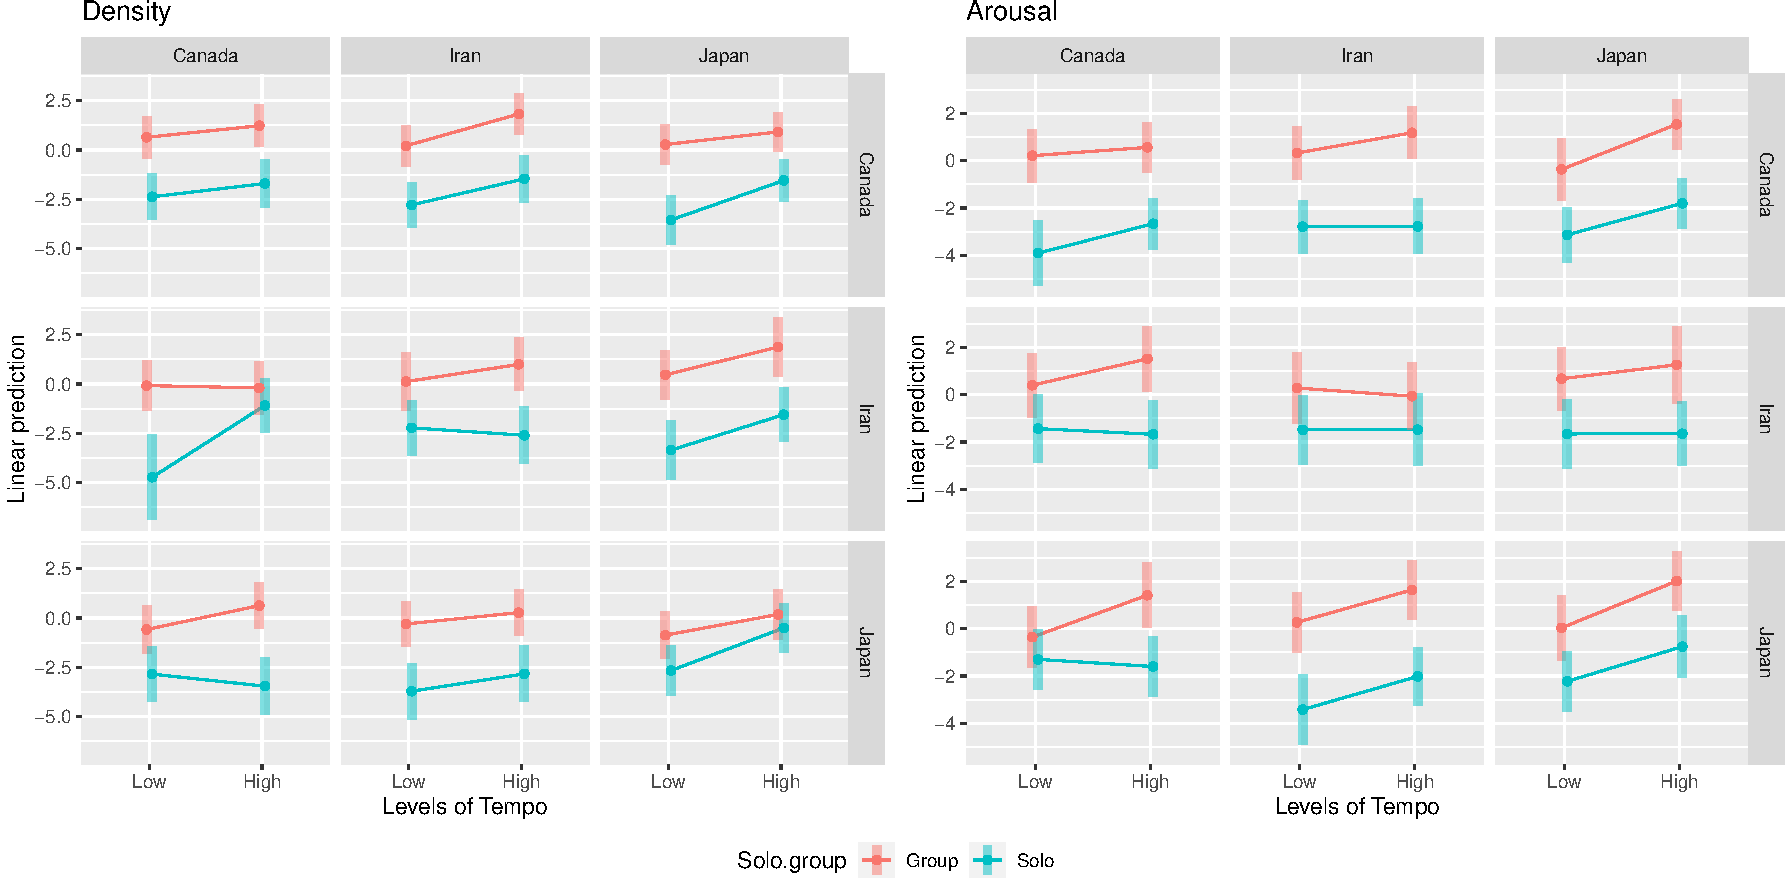
\includegraphics{Power_analysis_files/figure-latex/plot-mod-ex-1.pdf}
\caption{\label{fig:plot-mod-ex}Estimated marginal means and confidence intervals for the within-subject effects of Tempo from a ramdomly selected, simulated sample. Columns represent data from simulated participants from each country, while rows represent the simulated response to music from each country.}
\end{figure}

\hypertarget{effect-of-tempo}{%
\subsection{Effect of Tempo}\label{effect-of-tempo}}

Estimated marginal mean and contrast between the levels of Tempo (Low, High) averaged over the levels of instrumentation (\texttt{Solo.group}), participant country (\texttt{Participant.country}) and music country (\texttt{Music.country}). To obtain the estimated distributions of the ordinal levels of the dependent variable, the argument \texttt{mode\ =\ "mean.class"} can be added to the \texttt{emmeans} function \autocite[see][]{532079}.

\hypertarget{visual-density-model}{%
\subsubsection{Visual density model}\label{visual-density-model}}

Table of estimated marginal means and contrasts between tempo conditions. All estimated marginal means and contrasts were calculated using the \texttt{emmeans} function from the \texttt{emmeans} package \autocite{emmeanscit}.

\begin{Shaded}
\begin{Highlighting}[]
\FunctionTok{tempo.contr}\NormalTok{(model.den)}
\end{Highlighting}
\end{Shaded}

\begin{table}[H]

\caption{\label{tab:tab-den-emms}Estimated marginal means and contrasts between Tempo conditions}
\centering
\begin{threeparttable}
\begin{tabular}[t]{lccccclccc}
\toprule
\multicolumn{5}{c}{ } & \multicolumn{5}{c}{Contrasts} \\
\cmidrule(l{3pt}r{3pt}){6-10}
Tempo & EMM & $SE$ & $2.5\% CI$ & $97.5\% CI$ & Contrast & Difference & $SE$ & $z$ & $p$\\
\midrule
Low & -1.29 & 0.20 & -1.68 & -0.91 & Low - High & -0.95 & 0.25 & -3.8 & \textbf{< 0.001}\\
High & -0.34 & 0.21 & -0.75 & 0.07 &  &  &  &  & \\
\bottomrule
\end{tabular}
\begin{tablenotes}[para]
\item \textit{Note: } 
\item EMM = estimated marginal mean.
\end{tablenotes}
\end{threeparttable}
\end{table}

Figure of estimated marginal means and contrasts between tempo conditions.

\begin{Shaded}
\begin{Highlighting}[]
\FunctionTok{emmip}\NormalTok{(model.den, }\SpecialCharTok{\textasciitilde{}}\NormalTok{Tempo, }\AttributeTok{CIs =} \ConstantTok{TRUE}\NormalTok{)}
\end{Highlighting}
\end{Shaded}

\begin{figure}
\centering
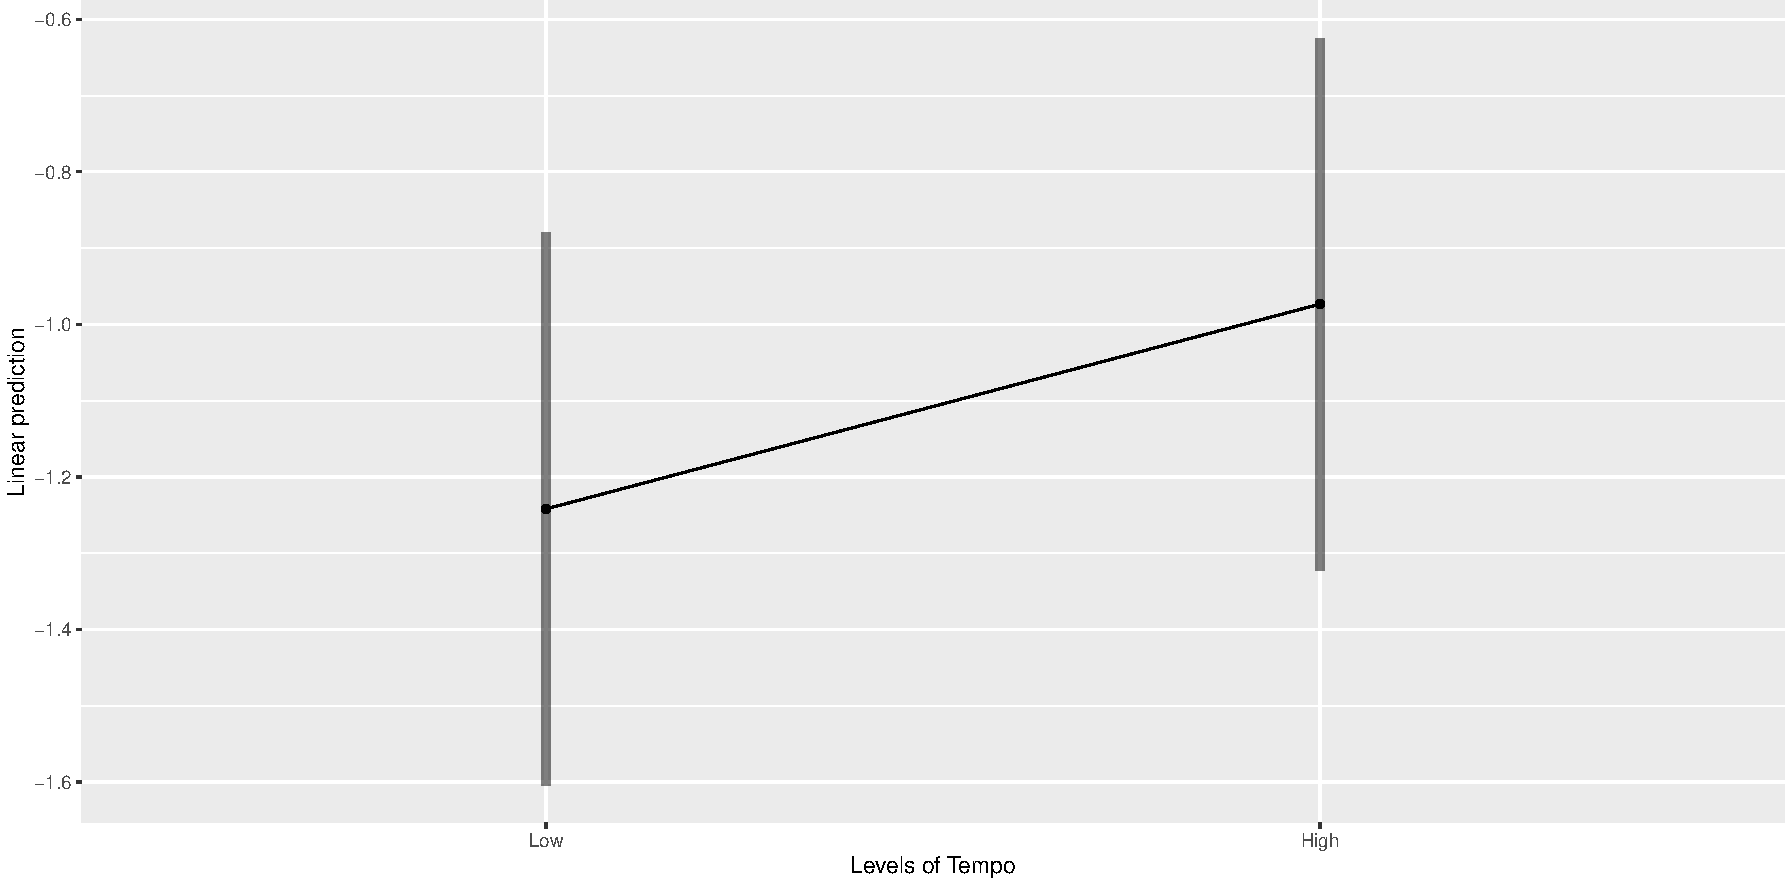
\includegraphics{Power_analysis_files/figure-latex/unnamed-chunk-18-1.pdf}
\caption{\label{fig:unnamed-chunk-18}Estimated marginal means and confidence intervals for the within-subject effects of Tempo on Visual density ratings, from a ramdomly selected, simulated sample, averaged across the levels of instrumentation, participant country and music country.}
\end{figure}

\hypertarget{arousal-model}{%
\subsubsection{Arousal model}\label{arousal-model}}

Table of estimated marginal means and contrasts between tempo conditions. All estimated marginal means and contrasts were calculated using the \texttt{emmeans} function from the \texttt{emmeans} package \autocite{emmeanscit}.

\begin{Shaded}
\begin{Highlighting}[]
\FunctionTok{tempo.contr}\NormalTok{(model.aro)}
\end{Highlighting}
\end{Shaded}

\begin{table}[H]

\caption{\label{tab:tab-aro-emms}Estimated marginal means and contrasts between Tempo conditions}
\centering
\begin{threeparttable}
\begin{tabular}[t]{lccccclccc}
\toprule
\multicolumn{5}{c}{ } & \multicolumn{5}{c}{Contrasts} \\
\cmidrule(l{3pt}r{3pt}){6-10}
Tempo & EMM & $SE$ & $2.5\% CI$ & $97.5\% CI$ & Contrast & Difference & $SE$ & $z$ & $p$\\
\midrule
Low & -1.43 & 0.22 & -1.86 & -1.00 & Low - High & -1.25 & 0.26 & -4.84 & \textbf{< 0.0001}\\
High & -0.19 & 0.16 & -0.51 & 0.14 &  &  &  &  & \\
\bottomrule
\end{tabular}
\begin{tablenotes}[para]
\item \textit{Note: } 
\item EMM = estimated marginal mean.
\end{tablenotes}
\end{threeparttable}
\end{table}

Figure of estimated marginal means and contrasts between tempo conditions.

\begin{Shaded}
\begin{Highlighting}[]
\FunctionTok{emmip}\NormalTok{(model.aro, }\SpecialCharTok{\textasciitilde{}}\NormalTok{Tempo, }\AttributeTok{CIs =} \ConstantTok{TRUE}\NormalTok{)}
\end{Highlighting}
\end{Shaded}

\begin{figure}
\centering
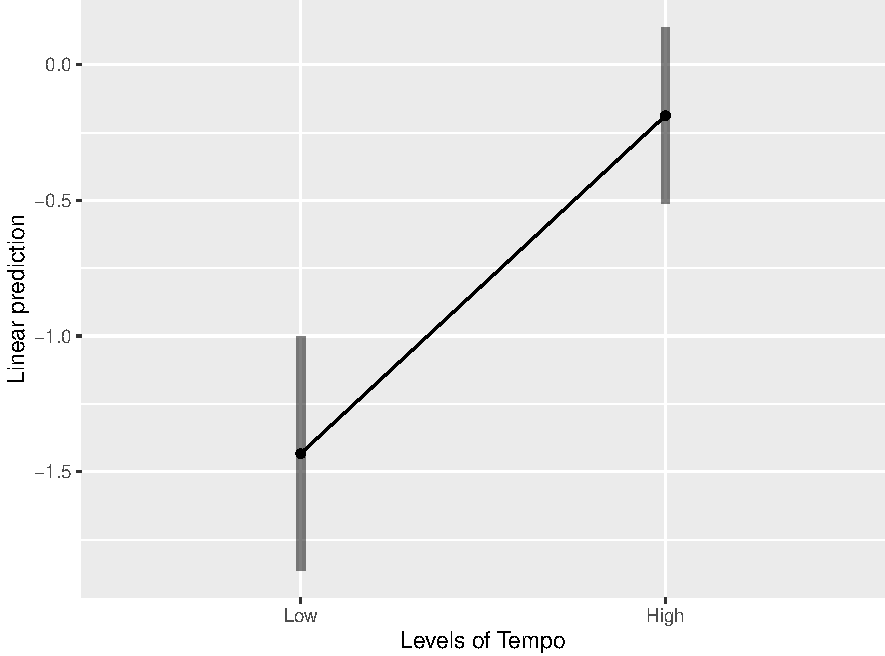
\includegraphics{Power_analysis_files/figure-latex/unnamed-chunk-19-1.pdf}
\caption{\label{fig:unnamed-chunk-19}Estimated marginal means and confidence intervals for the within-subject effects of Tempo on Arousal ratings, from a ramdomly selected, simulated sample, averaged across the levels of instrumentation, participant country and music country.}
\end{figure}

\hypertarget{conclusion}{%
\section{Conclusion}\label{conclusion}}

Based on the conducted power analysis (section \ref{power-section}), it can be inferred that a sample size of 24 participants per country (72 participants in total) would yield a statistical power (\(1 - \beta\)) greater than 0.95 for the planned contrasts between Tempo conditions when the effect size of this Tempo manipulation is 1. While the pilot data indicated a larger effect size, a conservative estimate was utilized to ensure sufficient statistical power even if the true effect size is significantly smaller than observed in the pilot study. This approach guarantees a high likelihood of correctly rejecting the null hypothesis in the presence of a true effect, providing confidence in the study's ability to detect meaningful findings.

In addition, as shown when fitting and reporting the models with a randomly selected sample (section \ref{example-data}), the sample size and data structure are adequate to fit the planned models.

\hypertarget{refs}{%
\section*{References}\label{refs}}
\addcontentsline{toc}{section}{References}

\begin{multicols}{2}
\AtNextBibliography{\footnotesize}
\printbibliography[heading=none]
\normalsize
\end{multicols}

\def\printbibliography{}

\hypertarget{session}{%
\section*{Session info (for reproducibility)}\label{session}}
\addcontentsline{toc}{section}{Session info (for reproducibility)}

\begin{Shaded}
\begin{Highlighting}[]
\FunctionTok{library}\NormalTok{(pander)}
\FunctionTok{pander}\NormalTok{(}\FunctionTok{sessionInfo}\NormalTok{(), }\AttributeTok{locale =} \ConstantTok{FALSE}\NormalTok{)}
\end{Highlighting}
\end{Shaded}

\textbf{R version 4.3.1 (2023-06-16 ucrt)}

\textbf{Platform:} x86\_64-w64-mingw32/x64 (64-bit)

\textbf{attached base packages:}
\emph{stats}, \emph{graphics}, \emph{grDevices}, \emph{utils}, \emph{datasets}, \emph{methods} and \emph{base}

\textbf{other attached packages:}
\emph{pander(v.0.6.5)}, \emph{beepr(v.1.3)}, \emph{scales(v.1.2.1)}, \emph{performance(v.0.10.4)}, \emph{kableExtra(v.1.3.4)}, \emph{ordinal(v.2022.11-16)}, \emph{emmeans(v.1.8.8)}, \emph{ggpubr(v.0.6.0)}, \emph{lubridate(v.1.9.2)}, \emph{forcats(v.1.0.0)}, \emph{stringr(v.1.5.0)}, \emph{dplyr(v.1.1.2)}, \emph{purrr(v.1.0.2)}, \emph{readr(v.2.1.4)}, \emph{tidyr(v.1.3.0)}, \emph{tibble(v.3.2.1)}, \emph{ggplot2(v.3.4.3)}, \emph{tidyverse(v.2.0.0)} and \emph{knitr(v.1.43)}

\textbf{loaded via a namespace (and not attached):}
\emph{tidyselect(v.1.2.0)}, \emph{viridisLite(v.0.4.2)}, \emph{farver(v.2.1.1)}, \emph{fastmap(v.1.1.1)}, \emph{TH.data(v.1.1-2)}, \emph{digest(v.0.6.33)}, \emph{estimability(v.1.4.1)}, \emph{timechange(v.0.2.0)}, \emph{lifecycle(v.1.0.3)}, \emph{survival(v.3.5-7)}, \emph{magrittr(v.2.0.3)}, \emph{compiler(v.4.3.1)}, \emph{rlang(v.1.1.1)}, \emph{tools(v.4.3.1)}, \emph{utf8(v.1.2.3)}, \emph{yaml(v.2.3.7)}, \emph{ggsignif(v.0.6.4)}, \emph{labeling(v.0.4.2)}, \emph{xml2(v.1.3.5)}, \emph{multcomp(v.1.4-25)}, \emph{abind(v.1.4-5)}, \emph{withr(v.2.5.0)}, \emph{numDeriv(v.2016.8-1.1)}, \emph{grid(v.4.3.1)}, \emph{fansi(v.1.0.4)}, \emph{xtable(v.1.8-4)}, \emph{colorspace(v.2.1-0)}, \emph{MASS(v.7.3-60)}, \emph{tinytex(v.0.46)}, \emph{insight(v.0.19.3)}, \emph{cli(v.3.6.1)}, \emph{mvtnorm(v.1.2-2)}, \emph{rmarkdown(v.2.24)}, \emph{generics(v.0.1.3)}, \emph{rstudioapi(v.0.15.0)}, \emph{httr(v.1.4.7)}, \emph{tzdb(v.0.4.0)}, \emph{audio(v.0.1-11)}, \emph{splines(v.4.3.1)}, \emph{rvest(v.1.0.3)}, \emph{vctrs(v.0.6.3)}, \emph{webshot(v.0.5.5)}, \emph{Matrix(v.1.6-1)}, \emph{sandwich(v.3.0-2)}, \emph{carData(v.3.0-5)}, \emph{bookdown(v.0.35)}, \emph{car(v.3.1-2)}, \emph{hms(v.1.1.3)}, \emph{rstatix(v.0.7.2)}, \emph{systemfonts(v.1.0.4)}, \emph{glue(v.1.6.2)}, \emph{codetools(v.0.2-19)}, \emph{cowplot(v.1.1.1)}, \emph{stringi(v.1.7.12)}, \emph{gtable(v.0.3.3)}, \emph{munsell(v.0.5.0)}, \emph{pillar(v.1.9.0)}, \emph{htmltools(v.0.5.6)}, \emph{R6(v.2.5.1)}, \emph{ucminf(v.1.2.0)}, \emph{evaluate(v.0.21)}, \emph{lattice(v.0.21-8)}, \emph{highr(v.0.10)}, \emph{backports(v.1.4.1)}, \emph{broom(v.1.0.5)}, \emph{Rcpp(v.1.0.11)}, \emph{svglite(v.2.1.1)}, \emph{coda(v.0.19-4)}, \emph{gridExtra(v.2.3)}, \emph{nlme(v.3.1-163)}, \emph{xfun(v.0.40)}, \emph{zoo(v.1.8-12)} and \emph{pkgconfig(v.2.0.3)}

\printbibliography

\end{document}
